% !TEX root = saveliev_physics_general_course_2.tex
%!TEX TS-program = pdflatex
%!TEX encoding = UTF-8 Unicode


\chapter[DIFFRACTION OF LIGHT]{DIFFRACTION OF LIGHT}\label{chap:18}
\chaptermark{DIFFRACTION OF LIGHT}

\section{Introduction}\label{sec:18_1}

By diffraction is meant the combination of phenomena observed when light propagates in a medium with sharp heterogeneities\footnote{For example, near the boundaries of opaque or transparent bodies, through small holes, etc.} and associated with deviations from the laws of geometrical optics.
Diffraction, in particular, leads to light waves bending around obstacles and to the penetration of light into the region of a geometrical shadow.
The bending of sound waves around obstacles (\ie, the diffraction of sound waves) is constantly observed in our everyday life.
To observe the diffraction of light waves, special conditions must be set up.
This is due to the smallness of the lengths of light waves.
We know that in the limit, when $\lambda\to 0$, the laws of wave optics transform into those of geometrical optics.
Hence, other conditions being equal, the deviations from the laws of geometrical optics decrease with a diminishing wavelength.

There is no appreciable physical difference between interference and diffraction.
Both phenomena consist in the redistribution of the light flux as a result of superposition of the waves.
For historical reasons, the redistribution of the intensity produced as a result of the superposition of waves emitted by a finite number of discrete coherent sources has been called the interference of waves.
The redistribution of the intensity produced as a result of the superposition of waves emitted by coherent sources arranged continuously has been called the diffraction of waves.
We, therefore, speak about the interference pattern from two narrow slits and about the diffraction pattern from one slit.

Diffraction is usually observed by means of the following set-up.
An opaque barrier closing part of the wave surface of the light wave is placed in the path of a light wave propagating from a certain source.
A screen on which the diffraction pattern appears is placed after the barrier.

Two kinds of diffraction are distinguished.
If the light source S and the point of observation P are so far from a barrier that the rays falling on the barrier and those travelling to point P form virtually parallel beams, we have to do with diffraction in parallel rays or with \textbf{Fraunhofer diffraction}.
Otherwise, we have to do with Fresnel diffraction.
Fraunhofer diffraction can be observed by placing a lens after light source S and another one in front of point of observation P, so that points S and P lie in the focal plane of the relevant lens
(\fig{18_1}).

The criterion allowing us to determine the kind of diffraction we are dealing with---Fresnel or Fraunhofer---in each specific case will be given in \sect{18_5}.

\begin{figure}[t]
	\begin{center}
		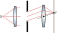
\includegraphics[scale=1]{figures/ch_18/fig_18_1.pdf}
		% \caption[]{}
        \caption[]{Fraunhofer diffraction observed by placing a lens after light source S and another one in front of point of observation P. Points S and P lie in the focal plane of each lens.}
		\label{fig:18_1}
	\end{center}
	\vspace{-0.8cm}
\end{figure}

\section{Huygens-Fresnel Principle}\label{sec:18_2}

The penetration of light waves into the region of a geometrical shadow can be explained with the aid of Huygens' principle (see \sect{16_9}).
This principle, however, gives no information on the amplitude and, consequently, on the intensity of waves propagating in different directions.
The French physicist Augustin Fresnel (1788-1827) supplemented Huygens' principle with the concept of the interference of secondary waves.
Taking into account the amplitudes and phases of the secondary waves makes it possible to find the amplitude of the resultant wave for any point of
space.
Huygens' principle developed in this way was named the \textbf{Huygens-Fresnel principle}.

According to the Huygens-Fresnel principle, every element of wave surface $S$ (\fig{18_2}) is the source of a secondary spherical wave whose amplitude is proportional to the size of element $\deriv{S}$.
The amplitude of a spherical wave diminishes with the distance $r$ from its source according to the law $1/r$ [see \eqn{14_12}].
Consequently, the oscillation
\begin{equation}\label{eq:18_1}
    \deriv{E} = K \frac{a_0\, \deriv{S}}{r} \cos(\omega t - kr + \alpha_0),
\end{equation}

\noindent
arrives from each section $\deriv{S}$ of a wave surface at point P in front of this surface.
In \eqn{18_1}, $(\omega t+\alpha_0)$ is the phase of the oscillation where wave surface $S$ is, $k$ is the wave number, $r$ is the distance from surface element $\deriv{S}$ to point P.
The factor $\alpha_0$ is determined by the amplitude of the light oscillation at the location of $\deriv{S}$.
The coefficient $K$ depends on the angle $\varphi$ between a normal $\hatvec{n}$ to area $\deriv{s}$ and the direction from $\deriv{S}$ to point P.
When $\varphi=0$, this coefficient is maximum; when $\varphi=\pi/2$, it vanishes.

\begin{figure}[t]
	\begin{center}
		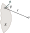
\includegraphics[scale=1]{figures/ch_18/fig_18_2.pdf}
		% \caption[]{}
        \caption[]{Huygens-Fresnel principle: every element of wave surface $S$ is the source of a secondary spherical wave whose amplitude is proportional to the size of element $\deriv{S}$.}
		\label{fig:18_2}
	\end{center}
	\vspace{-0.8cm}
\end{figure}

he resultant oscillation at point P is the superposition of the oscillations given by \eqn{18_1} taken for the entire wave surface $S$:
\begin{equation}\label{eq:18_2}
    E = \int_S K(\varphi) \frac{a_0}{r} \cos(\omega t - kr + \alpha_0)\, \deriv{S}.
\end{equation}

\noindent
This equation is an analytical expression of the Huygens-Fresnel principle.

The Huygens-Fresnel principle can be substantiated
by the following reasoning.
Assume that thin opaque screen Sc (\fig{18_3}) is
placed in the path of a light wave (we shall consider it plane for simplicity's sake).
The intensity of the light everywhere after the screen will be zero.
The reason is that the light wave falling on the screen produces oscillations of the electrons in the material of the screen.
The oscillating electrons emit electromagnetic waves.
The field after the screen is a superposition of the primary wave (falling on the screen) and all the secondary waves.
The amplitudes and phases of the secondary waves are such that upon superposition of these waves with the primary one, a zero amplitude is obtained at any point P after the screen.
Consequently, if the primary wave produces the oscillation
\begin{equation*}
    \ab{A}{prim} \cos(\omega t + \alpha)
\end{equation*}

\noindent
at point P, then the resultant oscillation produced by the secondary waves at the same point has the form
\begin{equation*}
    \ab{A}{sec} \cos(\omega t + \alpha - \pi).
\end{equation*}

\noindent
Here, $\ab{A}{sec}=\ab{A}{prim}$.

\begin{figure}[t]
	\begin{center}
		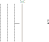
\includegraphics[scale=1]{figures/ch_18/fig_18_3.pdf}
		% \caption[]{}
        \caption[]{A light wave (primary wave) falling on a thin opaque screen Sc produces oscillations of the electrons in the material of the screen. The oscillating electrons emit electromagnetic waves (secondary wave). The amplitudes and phases of the secondary waves are such that, upon superposition of these waves with the primary one, a zero amplitude is obtained at any point P after the screen.}
		\label{fig:18_3}
	\end{center}
	\vspace{-0.8cm}
\end{figure}

What has been said above signifies that when calculating the amplitude of an oscillation set up at point P by a light wave propagating from a real source, we can replace this source with a collection of secondary sources arranged along the wave surface.
This is exactly the essence of Huygens-Fresnel principle.

Let us divide the opaque barrier into two parts.
One of them, which we shall call a stopper, has finite dimensions and an arbitrary shape (a circle, rectangle, etc.).
The other part includes the entire remaining surface of the infinite barrier.
As long as the stopper is in place, the resultant oscillation at point P after the barrier is zero.
It can be represented as the sum of the oscillations set up by the primary wave, the wave produced by the stopper, and the wave produced by
the remaining part of the barrier:
\begin{equation}\label{eq:18_3}
    \ab{A}{prim} \cos(\omega t+\alpha) + \ab{A}{stop} \cos(\omega t+\alpha') + \ab{A}{bar} \cos(\omega t+\alpha'') = 0.
\end{equation}

If the stopper is removed, \ie, the wave is transmitted through the aperture in the opaque barrier, then the oscillation at point P will have the form
\begin{align*}
    \ab{E}{P} &= \ab{A}{prim} \cos(\omega t+\alpha) + \ab{A}{bar} \cos(\omega t+\alpha'') \\
    &= - \ab{A}{stop} \cos(\omega t+\alpha') = \ab{A}{stop} \cos(\omega t+\alpha'-\pi).
\end{align*}

We have used condition \eqref{eq:18_3} and assumed that removal of the stopper does not change the nature of the oscillations of the electrons in the remaining part of the barrier.

We can, thus, consider that the oscillations at point P are produced by a collection of sources of secondary waves on the surface of the aperture formed after removal of the stopper.

\section{Fresnel Zones}\label{sec:18_3}

The performance of calculations by \eqn{18_2} is a very difficult task in the general case.
As Fresnel showed, however, the amplitude of the resultant oscillation can be found by simple algebraic or geometrical summation in cases distinguished by symmetry.

To understand the essence of the method developed by Fresnel, let us determine the amplitude of the light oscillation set up at point P by a spherical wave propagating in an isotropic homogeneous medium from point source S (\fig{18_4}).
The wave surfaces of such waves are symmetrical relative to straight line SP.
Taking advantage of this circumstance, let us divide the wave surface shown in the figure into annular zones constructed so that the distances from the edges of each zone to point P differ by $\lambda/2$ ($\lambda$ is the length of the wave
in the medium in which it is propagating).
Zones having this property are known as \textbf{Fresnel zones}.

\begin{figure}[t]
	\begin{center}
		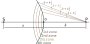
\includegraphics[scale=1]{figures/ch_18/fig_18_4.pdf}
		% \caption[]{}
        \caption[]{Fresnel zones obtained by division of a wave surface, travelling from S to P,  into annular zones constructed so that the distances from the edges of each zone to point P differ by $\lambda/2$, where $\lambda$ is the length of the wave in the medium of propagation.}
		\label{fig:18_4}
	\end{center}
	\vspace{-0.8cm}
\end{figure}

A glance at \fig{18_4} shows that the distance $b_m$ from the outer edge of the $m$-th zone to point P is
\begin{equation}\label{eq:18_4}
    b_m = b + m \frac{\lambda}{2}
\end{equation}

\noindent
($b$ is the distance from the crest $0$ of the wave surface to point P).

The oscillations arriving at point P from similar points of two adjacent zones (\ie, from points at the middle of the zones, or at the outer edges of the zones, etc.) are in counterphase.
Therefore, the resultant oscillations produced by each of the zones as a whole will differ in phase for adjacent zones by $\pi$ too.

Let us calculate the areas of the zones.
The outer boundary of the $m$-th zone separates a spherical segment of height $h_m$ on the wave surface (\fig{18_5}).
Let the area of this segment be $S_m$.
Hence, the area of the $m$-th zone can be written as
\begin{equation*}
    \Delta{S_m} = S_m - S_{m-1},
\end{equation*}

\noindent
where $S_{m-1}$ is the area of the spherical segment separated by the outer boundary of the $(m-1)$-th zone.

\begin{figure}[t]
	\begin{center}
		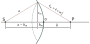
\includegraphics[scale=1]{figures/ch_18/fig_18_5.pdf}
		% \caption[]{}
        \caption[]{Area of a Fresnel zone. The outer boundary of the $m$-th zone separates a spherical segment of height $h_m$ on the wave surface. The area of this segment be $S_m$.}
		\label{fig:18_5}
	\end{center}
	\vspace{-0.8cm}
\end{figure}

It can be seen from \fig{18_5} that
\begin{equation*}
    r_m^2 = A^2 - (a - h_m)^2 = \parenthesis{b + m\frac{\lambda}{2}}^2 - \parenthesis{b + h_m}^2,
\end{equation*}

\noindent
where $a$ is the radius of the wave surface and $r_m$ is the radius of the outer boundary of the $m$-th zone.

Squaring the terms in parentheses, we get
\begin{equation}\label{eq:18_5}
    r_m^2 = 2ah_m - h_m^2 = bm\lambda + m^2\parenthesis{\frac{\lambda}{2}}^2 - 2bh_m - h_m^2,
\end{equation}

\noindent
whence,
\begin{equation}\label{eq:18_6}
    h_m = \frac{bm\lambda + m^2 (\lambda/2)^2}{2(a+b)}.
\end{equation}

\noindent
Restricting ourselves to a consideration of not too great $m$'s, we may disregard the addend containing $\lambda^2$ owing to the smallness of $\lambda$.
In this approximation
\begin{equation}\label{eq:18_7}
    h_m = \frac{bm\lambda}{2(a+b)}.
\end{equation}

The area of a spherical segment is $S=2\pi Rh$ (here, $R$ is the radius of the sphere and $h$ is the height of the segment).
Hence,
\begin{equation*}
    S_m = 2\pi a h_m = \bracket{\frac{\pi a b}{(a+b)}} m \lambda,
\end{equation*}

\noindent
and the area of the $m$-th zone is
\begin{equation*}
    \Delta{S_m} = S_m - S_{m-1} = \frac{\pi a b \lambda}{(a+b)}.
\end{equation*}

\noindent
The expression we have obtained does not depend on $m$.
This signifies that when $m$ is not too great, the areas of the Fresnel zones are approximately identical.

We can find the radii of the zones from \eqn{18_5}.
When $m$ is not too great, the height of a segment $h_m\ll a$, and we can, therefore, consider that $r_m^2= 2ah_m$.
Substituting for $h_m$ its value from \eqn{18_7},
we get the following expression for the radius of the outer boundary of the $m$-th zone:
\begin{equation}\label{eq:18_8}
    r_m = \bracket{ \parenthesis{ \frac{ab}{a+b} } m \lambda }^{1/2}.
\end{equation}

\noindent
If we assume that $a=b=\SI{1}{\metre}$ and $A=\SI{0.5}{\micro\metre}$, then, we get a value of $r_1=\SI{0.5}{\milli\metre}$ for the radius of the first (central) zone.
The radii of the following zones grow as $\sqrt{m}$.

Thus, the areas of the Fresnel zones are approximately the same.
The distance $b_m$ from a zone to point P slowly increases with the zone number $m$.
The angle $\varphi$ between a normal to the zone elements and the direction toward point P also grows with $m$.
All this leads to the fact that the amplitude $A_m$ of the oscillation produced by the $m$-th zone at point P diminishes monotonously with increasing $m$.
Even at very high values of $m$, when the area of a zone begins to grow appreciably with $m$ [see \eqn{18_6}], the decrease in the factor $K(\varphi)$ overbalances the increase in $\Delta{S_m}$, so that $A_m$ continues to diminish.
Thus, the amplitudes of the oscillations produced at point P by Fresnel zones form a monotonously diminishing sequence:
\begin{equation*}
    A_1 > A_2 > A_3 > \ldots > A_{m-1} > A_m > \ldots .
\end{equation*}

The phases of the oscillations produced by adjacent zones differ by $\pi$.
Therefore, the amplitude $A$ of the resultant oscillation at point P can be represented in the form
\begin{equation}\label{eq:18_9}
    A = A_1 - A_2 + A_3 - A_4 + \ldots .
\end{equation}

This expression includes all the amplitudes from odd zones with one sign and from even zones with the opposite one.

Let us write \eqn{18_9} in the form
\begin{equation}\label{eq:18_10}
	A = \frac{A_1}{2} + \parenthesis{ \frac{A_1}{2} - A_2 + \frac{A_3}{2} } + \parenthesis{ \frac{A_3}{2} - A_4 + \frac{A_5}{2} } + \ldots .
\end{equation}

\noindent
Owing to the monotonous diminishing of $A_m$, we can approximately assume that
\begin{equation*}
	A_m = \frac{A_{m-1} + A_{m+1}}{2}.
\end{equation*}

\noindent
The expressions in parentheses will therefore vanish, and \eqn{18_10} will be simplified as follows:
\begin{equation}\label{eq:18_11}
	A = \frac{A_1}{2}.
\end{equation}

\noindent
According to \eqn{18_11}, the amplitude produced at a point P by an entire spherical wave surface equals half the amplitude produced by the central zone alone.
If we put in the path of a wave an opaque screen having an aperture that leaves only the central Fresnel zone open, the amplitude at point P will equal $A_1$, \ie, it will be double the amplitude given by \eqn{18_11}.
Accordingly, the intensity of the light at point P will in this case be four times greater than when there are no barriers between points S and P.

Now, let us solve the problem on the propagation of light from source S to point P by the method of graphical addition of amplitudes.
We shall divide the wave surface into annular zones similar to Fresnel zones, but much smaller in width (the path difference from the edges of a zone to point P is a small fraction of $\lambda$ the same for all zones).
We shall depict the oscillation produced at point P by each of the zones in the form of a vector whose length equals the amplitude of the oscillation, while the angle made by the vector with the direction taken as the beginning of measurement gives the initial phase of the oscillation (see Sec. 7.7 of Vol. I).
The amplitude of the oscillations produced by such zones at point P slowly diminishes from zone to zone.
Each following oscillation lags behind the preceding one in phase by the same magnitude.
Hence, the vector diagram obtained when the oscillations produced by the separate zones are added has the form shown in \fig{18_6}.

\begin{figure}[t]
	\begin{minipage}[t]{0.48\linewidth}
		\begin{center}
			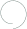
\includegraphics[scale=1]{figures/ch_18/fig_18_6.pdf}
			% \caption[]{}
            \caption[]{Vector diagram obtained when the oscillations produced by the separate zones are added. The vectors form a broken spiral-shaped line instead of a closed figure.}
			\label{fig:18_6}
		\end{center}
	\end{minipage}
	\hfill{ }%space{-0.05cm}
	\begin{minipage}[t]{0.48\linewidth}
		\begin{center}
			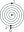
\includegraphics[scale=1]{figures/ch_18/fig_18_7.pdf}
            % \caption[]{}
			\caption[]{The phases of the oscillations at points $0$ and $1$ differ by $\pi$ (the infinitely small vectors forming the spiral have opposite directions at these points).}
			\label{fig:18_7}
		\end{center}
	\end{minipage}
\vspace{-0.4cm}
\end{figure}

If the amplitudes produced by the individual zones were the same, the tail of the last of the vectors shown in \fig{18_6} would coincide with the tip of the first vector.
Actually, the value of the amplitude diminishes, although very slightly.
Hence, the vectors form a broken spiral-shaped line instead of a closed figure.

In the limit when the widths of the annular zones tend to zero (their number will grow unlimitedly), the vector diagram has the form of a spiral winding toward point C (\fig{18_7}).
The phases of the oscillations at points $0$ and $1$ differ by $\pi$ (the infinitely small vectors forming the spiral have opposite directions at these points).

Consequently, part $0$-$1$ of the spiral corresponds to the first Fresnel zone.
The vector drawn from point $0$ to point $1$ (\fig{18_8}a) depicts the oscillation produced at point P by this zone.
Similarly, the vector drawn from point $1$ to point $2$ (\fig{18_8}b) depicts the oscillation produced by the second Fresnel zone.
The oscillations from the first and second zones are in counterphase; accordingly, vectors $01$ and $12$ have opposite directions.

The oscillation produced at point P by the entire wave surface is depicted by vector $0$C (\fig{18_8}c).
Inspection of the figure shows that the amplitude in this case equals half the amplitude produced
by the first zone.
We have obtained this result algebraically earlier [see \eqn{18_11}].
We shall note that the oscillation produced by the
inner half of the first Fresnel zone is depicted by vector $0$B (\fig{18_8}d).
Thus, the action of the inner half of the first Fresnel zone is not equivalent to half the action of the first zone.
Vector $0$B is $\sqrt{2}$ times greater than vector $0$C.
Consequently, the intensity of the light produced by the inner half of the first Fresnel zone is double the intensity produced by the entire wave surface.

\begin{figure}[t]
	\begin{center}
		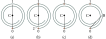
\includegraphics[scale=0.9]{figures/ch_18/fig_18_8.pdf}
		% \caption[]{}
        \caption[]{(a, b) First and second Fresnel zones. (c) The oscillation produced at point P by the entire wave surface is depicted by vector OC. The amplitude here equals half the amplitude produced by the first zone. (d) The oscillation produced by the inner half of the first Fresnel zone is depicted by vector $0$B, which is $\sqrt{2}$ times greater than vector $0$C. Thus, the intensity of light in the inner half of the First zone is twice that of the entire wave surface.}
		\label{fig:18_8}
	\end{center}
	\vspace{-0.8cm}
\end{figure}

The oscillations from the even and odd Fresnel zones are in counterphase and, therefore, mutually weaken one another.
If we would place in the path of the light wave a plate that would cover all the even or odd zones, the intensity of the light at point P would sharply grow.
Such a plate, known as a zone one, functions like a converging lens.
Figure \ref{fig:18_9} shows a plate covering the
even zones.
A still greater effect can be achieved by changing the phase of the even (or odd) zone oscillations by $\pi$ instead of covering these
zones.
This can be done with the aid of a transparent plate whose thickness at the places corresponding
to the even or odd zones differs by a properly selected value.
Such a plate is called a \textbf{phase zone plate}.
In comparison with the \textbf{amplitude zone plate} covering zones, a phase plate produces an additional two-fold increase in the amplitude, and a four-fold increase in the light intensity.

\begin{figure}[t]
	\begin{center}
		
\includegraphics[scale=1]{figures/ch_18/fig_18_9.pdf}
		% \caption[]{}
        \caption[]{Plate covering the even Fresnel zones. The oscillations from the even and odd Fresnel zones are in counterphase and, therefore, mutually weaken one another.}
		\label{fig:18_9}
	\end{center}
	\vspace{-0.8cm}
\end{figure}

\section{Fresnel Diffraction from Simple Barriers}\label{sec:18_4}

The methods of algebraic and graphical addition of amplitudes treated in the preceding section make it possible to solve a number of problems involving the diffraction of light.

\textbf{Diffraction from a Round Aperture.}
Let us put an opaque screen with a round aperture of radius $r_0$ cut out in it in the path of a spherical light wave.
We shall arrange the screen so that a perpendicular dropped from light source S passes through the centre of the aperture (\fig{18_10}).
Let us take point P on the continuation of this perpendicular.
At an aperture radius $r_0$ considerably smaller than the lengths $a$ and $b$ shown in the figure, the length $a$ can be considered equal to the distance from source S to the barrier, and the length $b$, to the distance from the barrier to point P.
If the distances $a$ and $b$ satisfy the relation
\begin{equation}\label{eq:18_12}
	r_0 = \bracket{ \parenthesis{ \frac{ab}{a+b} } m \lambda }^{1/2},
\end{equation}

\noindent
where $m$ is an integer, then the aperture will leave open exactly $m$ first Fresnel zones constructed for point P [see \eqn{18_8}].
Hence, the number of open Fresnel zones is determined by the expression
\begin{equation}\label{eq:18_13}
	m = \frac{r_0^2}{\lambda} \parenthesis{\frac{1}{a} + \frac{1}{b}}.
\end{equation}

\begin{figure}[t]
	\begin{center}
		\includegraphics[scale=1]{figures/ch_18/fig_18_10.pdf}
		% \caption[]{}
        \caption[]{Opaque screen with a round aperture of radius $r_0$ cut out in it in the path of a spherical light wave. The screen is arranged so that a perpendicular dropped from light source S passes through the centre of the aperture. The diffraction patterns produced by the round aperture are shown for when $m$ is odd (b) and when $m$ is even (c).}
		\label{fig:18_10}
	\end{center}
	\vspace{-0.8cm}
\end{figure}

According to \eqn{18_9}, the amplitude at point P will be
\begin{equation}\label{eq:18_14}
	A = A_1 - A_2 + A_3 - A_4 + \ldots \pm A_m.
\end{equation}

\noindent
The amplitude $A_m$ is taken with a plus sign if $m$ is odd and with a minus sign if $m$ is even.
Writing \eqn{18_14} in a form similar to \eqn{18_10} and assuming that the expressions in parentheses equal zero, we arrive at the equations
\begin{align*}
	A &= \frac{A_1}{2} + \frac{A_m}{2} \quad \text{($m$ is odd)}\\
	A &= \frac{A_1}{2} + \frac{A_{m-1}}{2} - A_m \quad \text{($m$ is even)}.
\end{align*}

\noindent
The amplitudes from two adjacent zones are virtually the same.
We may therefore replace $(A_{m-1}/2)-A_m$ with $-A_m/2$.
The result is
\begin{equation}\label{eq:18_15}
	A = \frac{A_1}{2} \pm \frac{A_m}{2},
\end{equation}

\noindent
where the plus sign is taken for odd and the minus sign for even $m$'s.

The amplitude $A_m$ differs only slightly from $A_1$ for small $m$'s.
Hence, with odd $m$'s, the amplitude at point P will approximately equal $A_1$, and at even $m$'s, zero.
It is easy to obtain this result with the aid of the vector diagram shown in \fig{18_7}.

If we remove the barrier, the amplitude at point P will become equal to $A_1/2$ [see \eqn{18_11}].
Thus, a barrier with an aperture opening a small odd number of zones not only does not weaken the illumination at point P but, on the contrary, leads to an increase in the amplitude almost twice, and of the intensity, almost four
times.

Let us determine the nature of the diffraction pattern that will be observed on a screen placed after the barrier (see \fig{18_10}).
Owing to the symmetrical arrangement of the aperture relative to straight line SP, the illumination at various points of the screen will depend only on the distance $r$ from point P.
At this point itself, the intensity will reach a maximum or a minimum depending on whether the number of open (effective) Fresnel zones is even or odd.
Assume, for example, that this number is three.
In this case, we get a maximum of intensity at the centre of the diffraction pattern.
A pattern of the Fresnel zones for point P is given in \fig{18_11}a.

\begin{figure}[t]
	\begin{center}
		
\includegraphics[scale=1]{figures/ch_18/fig_18_11.pdf}
		% \caption[]{}
        \caption[]{(a, b, c) Diffraction patterns for different numbers of Fresnel zones obtained at points P, P$'$, and P$''$ of \fig{18_10}a, respectively. The patterns in (b) and (c) are limited by the edges of the aperture.}
		\label{fig:18_11}
	\end{center}
	\vspace{-0.8cm}
\end{figure}

Now let us move along the screen to point P$'$.
The pattern of the Fresnel zones for point P$'$ limited by the edges of the aperture has the form shown in \fig{18_11}b.
The edges of the aperture will obstruct a part of the third zone, and simultaneously the fourth zone will be partly opened.
As a result, the intensity of the light diminishes, and reaches a minimum at a certain position of point P$'$.
If we move along the screen to point P$''$, the edges of the aperture will partly obstruct not only the third, but also the second Fresnel zone, simultaneously partly opening the fifth zone (\fig{18_11}c).
The result will be that the action of the open sections of the odd zones will overbalance the action of the open sections of the even zones and the intensity will reach a maximum.
True, this maximum will be weaker than that observed at point P.

Thus, the diffraction pattern produced by a round aperture has the form of alternating bright and dark concentric rings.
There will be either a bright ($m$ is odd) or a dark ($m$ is even) spot at the centre of the pattern (\fig{18_12}).
The variation in the intensity $I$ with the distance $r$ from the centre of the pattern is shown in \fig{18_10}b (for an odd $m$) and in \fig{18_10}c (for an even $m$).
When the screen is moved parallel to itself along straight line SP, the patterns shown in \fig{18_12} will replace one another [according to \eqn{18_13}, when $b$ changes, the value of $m$ becomes odd and even alternately].

\begin{figure}[t]
	\begin{center}
		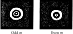
\includegraphics[scale=0.9]{figures/ch_18/fig_18_12.pdf}
		% \caption[]{}
        \caption[]{Diffraction patterns produced by a round aperture alternating bright and dark concentric rings. At the centre of the pattern, a bright spot results for an odd $m$ value, while a dark spot for an even $m$.}
		\label{fig:18_12}
	\end{center}
	\vspace{-0.8cm}
\end{figure}

If the aperture opens only a part of the central Fresnel zone, a blurred bright spot is obtained on the screen; there is no alternation of bright and dark rings in this case.
If the aperture opens a great number of zones, the alternation of the bright and dark rings is observed only in a very narrow region on the boundary of the geometrical shadow; inside this region the illumination is virtually constant.

\textbf{Diffraction from a Disk.}
Let us place an opaque disk of radius $r_0$ between light source S and observation point P (\fig{18_13}).
If the disk covers $m$ first Fresnel zones, the amplitude at point P will be
\begin{equation*}
	A = A_{m+1} - A_{m+2} + A_{m+3} - \ldots = \frac{A_{m+1}}{2} + \parenthesis{ \frac{A_{m+1}}{2} - A_{m+2} + \frac{A_{m+3}}{2} } + \ldots .
\end{equation*}

\noindent
The expressions in parentheses can be assumed to equal zero, consequently
\begin{equation}\label{eq:18_16}
	A = \frac{A_{m+1}}{2}.
\end{equation}

Let us determine the nature of the pattern obtained on the screen (see \fig{18_13}).
It is obvious that the illumination can depend only on the distance $r$ from point P.
With a small number of covered zones, the amplitude $A_{m+1}$ differs slightly from $A_1$.
The intensity at point P will therefore be almost the same as in the absence of a barrier between source S and point P [see \eqn{18_11}].
For point P$'$, displaced relative to point P in any radial direction, the disk will cover a part of the $(m+1)$-th Fresnel zone and part of the
$m$-th zone will be opened simultaneously.
This will cause the intensity to diminish.
At a certain position of point P$'$, the intensity will reach its minimum.
If the distance from the centre of the pattern is still greater, the disk will cover additionally a part of the $(m+2)$-th zone, and a part of the $(m-1)$-th zone will be opened simultaneously.
As a result, the intensity grows and reaches a
maximum at point P$''$.

\begin{figure}[t]
	\begin{minipage}[t]{0.6\linewidth}
		\begin{center}
			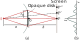
\includegraphics[scale=0.9]{figures/ch_18/fig_18_13.pdf}
			% \caption[]{}
            \caption[]{(a) Opaque disk of radius $r_0$ between light source S and observation point P. (b) Variation of the light intensity with the distance $r$ from point P.}
			\label{fig:18_13}
		\end{center}
	\end{minipage}
	\hfill{ }%space{-0.05cm}
	\begin{minipage}[t]{0.34\linewidth}
		\begin{center}
			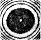
\includegraphics[scale=0.9]{figures/ch_18/fig_18_14.pdf}
            % \caption[]{}
			\caption[]{Diffraction pattern for an opaque disk alternating bright and dark concentric rings.}
			\label{fig:18_14}
		\end{center}
	\end{minipage}
\vspace{-0.4cm}
\end{figure}

Thus, the diffraction pattern for an opaque disk has the form of alternating bright and dark concentric rings.
The centre of the pattern contains a bright spot (\fig{18_14}).
The light intensity $I$ varies with the distance $r$ from point P as shown in \fig{18_13}b.

If the disk covers only a small part of
\fig{18_14} the central Fresnel zone, it does not form a shadow at all---the illumination of the screen everywhere is the same as in the absence of barriers.
If the disk covers many Fresnel zones, alternation of the bright and dark rings is observed only in a narrow region on the boundary of the geometrical shadow.
In this case, $A_{m+1}\ll A_1$, so that the bright spot at the centre is absent, and the illumination in the region of the geometrical shadow equals zero practically everywhere.

The bright spot at the centre of the shadow formed by a disk was the cause of an incident between Simeon Poisson and Augustin Fresnel.
The Paris Academy of Sciences announced the diffraction of light as the topic for its 1818 prize.
The organizers of the competition were advocates of the corpusculate theory of light and were sure that the papers submitted to the competition would bring a final victory to their theory.
Fresnel submitted a paper, however, in which all the optical phenomena known at that time were explained from the wave viewpoint.
In considering this paper, Poisson, who was a member of the competition committee, gave attention to the fact that an ``absurd'' conclusion follows from Frenel's theory: there must be a bright spot at the centre of the shadow formed by a small disk.
D. Arago immediately conducted an experiment and
found that such a spot does indeed exist.
This brought victory and all-round recognition to the wave theory of light.

\textbf{Diffraction from the Straight Edge of a Half-Plane.}
Let us put an opaque half-plane with a straight edge in the path of a light wave (which we shall consider to be plane for simplicity).
We shall arrange this half-plane so that it coincides with one of the wave surfaces.
We shall place a screen parallel to the half plane at a distance $b$ behind it and take point P on the screen (\fig{18_15}).
Let us divide the open part of the wave surface into zones having the form of very narrow straight strips parallel to the edge of the half-plane.
We shall choose the width of the zones so that the distances from point P to the edges of any zone measured in the plane of the drawing differ by the same amount $\Delta$.
When this condition is observed, the oscillations set up at point P by the adjacent zones will differ in phase by a constant value.

We shall assign the numbers $1$, $2$, $3$, etc. to the zones at the right of point P, and the numbers $1'$, $2'$, $3'$, etc. to those at the left of this point.
The zones numbered $m$ and $m'$ have an identical width and are symmetrical relative to point P.
Therefore, the oscillations produced by them at P coincide in amplitude and in phase.

\begin{figure}[t]
	\begin{minipage}[t]{0.58\linewidth}
		\begin{center}
			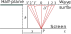
\includegraphics[scale=0.95]{figures/ch_18/fig_18_15.pdf}
			% \caption[]{}
            \caption[]{Opaque half-plane with a straight edge in the path of a light wave, arranged to coincide with one of the wave surfaces. A screen parallel to the half-plane is at a distance $b$ behind it.}
			\label{fig:18_15}
		\end{center}
	\end{minipage}
	\hfill{ }%space{-0.05cm}
	\begin{minipage}[t]{0.38\linewidth}
		\begin{center}
			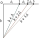
\includegraphics[scale=0.95]{figures/ch_18/fig_18_16.pdf}
            % \caption[]{}
			\caption[]{Picture that helps to establish the dependence of the amplitude on the zone number $m$.}
			\label{fig:18_16}
		\end{center}
	\end{minipage}
\vspace{-0.4cm}
\end{figure}

To establish the dependence of the amplitude on the zone number $m$, let us assess the areas of the zones.
A glance at \fig{18_16} shows that the total width of the first $m$ zones is
\begin{equation*}
	d_1 + d_2 + \ldots + d_m = \sqrt{(b+m\Delta)^2 - b^2} = \sqrt{2bm\Delta + m^2\Delta^2}.
\end{equation*}

\noindent
Since the zones are narrow, we have $\Delta\ll b$.
Consequently, when $m$  is not very great, we may ignore the quadratic term in the radicand.
This yields
\begin{equation*}
	d_1 + d_2 + \ldots + d_m = \sqrt{2bm\Delta}.
\end{equation*}

\noindent
Assuming in this equation that $m=1$, we find that $d_1=\sqrt{2b\Delta}$.
Hence, we can write the expression for the total width of the first $m$ zones as follows
\begin{equation*}
	d_1 + d_2 + \ldots + d_m = \sqrt{m},
\end{equation*}

\noindent
whence
\begin{equation}\label{eq:18_17}
	d_m = d_1 \parenthesis{ \sqrt{m} - \sqrt{m-1} }.
\end{equation}

Calculations by \eqn{18_17} show that
\begin{equation}\label{eq:18_18}
	d_1 : d_2 : d_3 : d_4 : \ldots = 1 : 0.41 : 0.32 : 0.27 : \ldots .
\end{equation}

\noindent
The areas of the zones are in the same proportion.
Examination of \eqn{18_18} shows that the amplitude of the oscillations set up at point P by the individual zones initially (for the first zones) diminishes very rapidly, and then this diminishing becomes slower.
For this reason, the broken line obtained in the graphical addition of the oscillations produced by the straight zones first has a gentler slope than that for annular zones (the areas of which in a similar construction are approximately equal).
Both vector diagrams are compared in \fig{18_17}.
In both cases, the lag in phase of each following oscillation has been taken the same.
The value of the amplitude for the annular zones (\fig{18_17}a) has been taken constant, and for the straight zones (\fig{18_17}b), diminishing
in accordance with proportion (\fig{18_18}).
The graphs in \fig{18_17} are approximate.
In an exact construction of these graphs, account must be taken of the dependence of the amplitude on $r$ and $\varphi$ [see \eqn{18_1}].
This does not affect the general nature of the diagrams, however.

\begin{figure}[t]
	\begin{minipage}[t]{0.48\linewidth}
		\begin{center}
			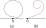
\includegraphics[scale=1]{figures/ch_18/fig_18_17.pdf}
			% \caption[]{}
            \caption[]{Approximate vector diagrams showing the graphical addition of the oscillations produced by straight lines. The amplitudes are constant in (a) and variable in accordance to \eqn{18_18} in (b).}
			\label{fig:18_17}
		\end{center}
	\end{minipage}
	\hfill{ }%space{-0.05cm}
	\begin{minipage}[t]{0.48\linewidth}
		\begin{center}
			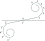
\includegraphics[scale=1]{figures/ch_18/fig_18_18.pdf}
            % \caption[]{}
			\caption[]{Complete diagram vectors depicting the oscillations corresponding to these zones symmetrically relative to the origin of coordinates $0$.}
			\label{fig:18_18}
		\end{center}
	\end{minipage}
\vspace{-0.4cm}
\end{figure}

Figure \fig{18_17}b shows only the oscillations produced by the zones to the right of point P.
The zones numbered $m$ and $m'$ are symmetrical relative to P.
It is therefore natural, when constructing the diagram, to arrange the vectors depicting the oscillations corresponding to these zones symmetrically relative to the origin of coordinates $0$ (\fig{18_18}).
If the width of the zones is made to tend to zero, the broken line shown in \fig{18_18} will transform into a smooth curve (\fig{18_19}) called a \textbf{Cornu spiral}.

The equation of a Cornu spiral in the parametric form is
\begin{equation}\label{eq:18_19}
	\xi = \int_0^v \cos\parenthesis{\frac{\pi u^2}{2}}\, \deriv{u}, \quad \eta = \int_0^v \sin\parenthesis{\frac{\pi u^2}{2}}\, \deriv{u}.
\end{equation}

\begin{figure}[t]
	\begin{center}
		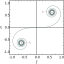
\includegraphics[scale=1]{figures/ch_18/fig_18_19.pdf}
		% \caption[]{}
        \caption[]{Cornu spiral. When the width of the zones is made tend to zero, the broken line shown in \fig{18_18} transforms into a smooth curve. This makes it possible to find the amplitude of a light oscillation at any point on a screen.}
		\label{fig:18_19}
	\end{center}
	\vspace{-0.8cm}
\end{figure}

\noindent
These integrals are known as Fresnel integrals.
They can be solved only numerically, and tables are available that can be used to find the values of the integrals for various $v$'s.
The meaning of the parameter $v$ is that $|v|$ gives the length of the arc of the Cornu spiral measured from the origin of coordinates.

The figures along the curve in \fig{18_19} give the values of the parameter $v$.
Points F$_1$ and F$_2$, which are asymptotically approached by the curve when $v$ tends to $+\infty$ and $-\infty$, are called the \textbf{focal points} or \textbf{poles} of the Cornu spiral.
Their coordinates are
\begin{align*}
	\xi &= + \frac{1}{2}, \quad \eta = + \frac{1}{2}, \quad \text{for point F$_1$},\\
	\xi &= - \frac{1}{2}, \quad \eta = - \frac{1}{2}, \quad \text{for point F$_2$}.
\end{align*}

\noindent
The right-hand curl of the spiral (section $0$F$_1$) corresponds to zones to the right of point P, and the left-hand curl (section $0$F$_2$) to zones to the left of this point.

Let us find the derivative $\diffin{\eta}{\xi}$ for the point of the curve corresponding to a given value of the parameter $v$.
According to \eqn{18_19}, the values
\begin{equation*}
	\deriv{\xi} = \cos\parenthesis{\frac{\pi v^2}{2}}\, \deriv{v}\, \quad \deriv{\eta} = \sin\parenthesis{\frac{\pi v^2}{2}}\, \deriv{v},
\end{equation*}

\noindent
correspond to the increment $\deriv{x}$ of $v$.
Consequently, $\diffin{\eta}{\xi}=\tan(\pi v^2/2)$.
At the same time, $\diffin{\eta}{\xi}= \tan\theta$, where $\theta$ is the angle of inclination of a tangent to the curve at the given point.
Thus,
\begin{equation}\label{eq:18_20}
	\theta = \frac{\pi}{2} v^2.
\end{equation}

\noindent
It thus follows that at the point corresponding to $v=1$ a tangent to the Cornu spiral is perpendicular to the $\xi$-axis.
When $v=2$, the angle $\theta$ is $2\pi$, so that a tangent is parallel to the $\xi$-axis.
When $v=3$, the angle $\theta$ is $9\pi/2$, so that a tangent is again perpendicular to the $\xi$-axis, and so on.

\begin{figure}[t]
	\begin{center}
		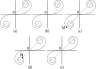
\includegraphics[scale=1]{figures/ch_18/fig_18_20.pdf}
		% \caption[]{}
        \caption[]{(a) The right-hand curl of the spiral corresponds to oscillations from the unhatched zones depicted by a vector whose origin is at point 0 and whose end is at point F$_1$. (b) When point P is displaced to the region of the geometrical shadow, the half-plane covers a greater and greater number of unhatched zones. The beginning of the resultant vector moves along the right-hand curl in the direction of pole F$_1$. If point P is displaced from the boundary of the geometrical shadow to the right, the tip of the resultant vector slides along the left-hand curl of the spiral in a direction to pole F$_2$. The amplitude passes through a number of maxima [the first one equals the length of the segment MF$_1$ (c)] and minima [the first one equals the length of segment NF$_1$ (d)]. }
		\label{fig:18_20}
	\end{center}
	\vspace{-0.8cm}
\end{figure}

The Cornu spiral makes it possible to find the amplitude of a light oscillation at any point on a screen.
We shall characterize the position of the point by the coordinate $x$ measured from the boundary of the geometrical shadow (see \fig{18_15}).
All the hatched zones will be covered for point P on the boundary of the geometrical shadow ($x=0$).
The right-hand curl of the spiral corresponds to oscillations from the unhatched zones.
Hence, the resultant oscillation will be depicted by a vector whose origin is at point $0$ and whose end is at point F$_1$ (\fig{18_20}a).
When point P is displaced to the region of the geometrical shadow, the half-plane covers a greater and greater number of unhatched zones.
Therefore, the beginning of the resultant vector moves along the right-hand curl in the direction of pole F$_1$ (\fig{18_20}b).
As a result, the amplitude of the oscillation monotonously tends to zero.

If point P is displaced from the boundary of the geometrical shadow to the right, in addition to the unhatched zones a constantly growing number of hatched ones will be uncovered.
Therefore, the tip of the resultant vector slides along the left-hand curl of the spiral in a direction to pole F$_2$.
The amplitude passes through a number of maxima (the first of them equals the length of segment MF$_1$ in \fig{18_20}c) and minima (the first of them equals the length of segment NF$_1$ in \fig{18_20}d).
When the wave surface is completely uncovered, the amplitude equals the length of F$_2$F$_1$ (\fig{18_20}e), \ie, is exactly double the amplitude on the boundary of the geometrical shadow (see \fig{18_20}a).
Accordingly, the intensity on the boundary of the geometrical shadow is one-fourth of the intensity $I_0$ obtained on the screen in the absence of barriers.

\begin{figure}[t]
	\begin{minipage}[t]{0.54\linewidth}
		\begin{center}
			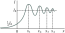
\includegraphics[scale=0.95]{figures/ch_18/fig_18_21.pdf}
			% \caption[]{}
            \caption[]{Dependence of light intensity with the coordinate $x$. Upon a transition to the region of the geometrical shadow, the intensity gradually tends to zero instead of changing in a jump. A number of alternating maxima and minima of the intensity are to the right of the boundary of the geometrical shadow.}
			\label{fig:18_21}
		\end{center}
	\end{minipage}
	\hfill{ }%space{-0.05cm}
	\begin{minipage}[t]{0.42\linewidth}
		\begin{center}
			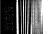
\includegraphics[scale=0.95]{figures/ch_18/fig_18_22.pdf}
            % \caption[]{}
			\caption[]{Photograph of the diffraction pattern produced by the edge of a half-plane.}
			\label{fig:18_22}
		\end{center}
	\end{minipage}
\vspace{-0.4cm}
\end{figure}

The dependence of light intensity $I$ on the coordinate $z$ is shown in \fig{18_21}.
Inspection of the figure shows that upon a transition to the region of the geometrical shadow, the intensity gradually tends to zero instead of changing in a jump.
A number of alternating maxima and minima of the intensity are to the right of the boundary of the geometrical shadow.
Calculations show that at $b=\SI{1}{\metre}$ and $\lambda=\SI{0.5}{\micro\metre}$ the coordinates of the maxima (see \fig{18_21}) have the following values: $x_1=\SI{0.61}{\milli\metre}$, $x_2=\SI{1.17}{\milli\metre}$, $x_3=\SI{1.54}{\milli\metre}$, $x_4=\SI{1.85}{\milli\metre}$, etc.
With a change in the distance $b$ from the half-plane to the screen, the values of the coordinates of the maxima and minima vary as $\sqrt{b}$.
It can be seen from the above data that the maxima are quite dense.
The Cornu curve can also be used to find the relative value of the intensity at the maxima and
minima.
We get the value of $1.37 I_0$ for the first maximum and $0.78 I_0$ for the first minimum.

Figure \ref{fig:18_22} contains a photograph of the diffraction pattern produced by the edge of a half-plane.

\textbf{Diffraction from a Slit.}
An infinitely long slit can be formed by placing two half-planes facing opposite directions next to each other.
Therefore, the problem on the Fresnel diffraction from a slit can be solved with the aid of a Cornu spiral.
We shall consider that the wave surface of the incident light, the plane of the slit, and the screen on which a diffraction pattern is observed are parallel to one another (\fig{18_23}).

For point P opposite the middle of the slit, the tip and the tail of the resultant vector are at points on the spiral that are symmetrical relative to the origin of coordinates (\fig{18_24}).
If we move to point P' opposite an edge of
the slit, the tip of the resultant vector
will move to the middle of the spiral $0$.
The tail of the vector will move along the spiral in the direction of pole F$_1$.
Upon motion into the region of the geometrical shadow, the tip and the tail of the resultant vector will slide along the spiral and in the long run will be at the smallest distance apart (see the vector in \fig{18_24} corresponding to point P$''$).
The intensity of the light reaches a minimum here.
Upon further sliding along the spiral, the tip and tail of the vector will move apart again, and the intensity will grow.
The same will occur when we move from point P in the opposite direction because the diffraction pattern is symmetrical relative to the middle of the slit.

\begin{figure}[t]
	\begin{minipage}[t]{0.48\linewidth}
		\begin{center}
			\includegraphics[scale=1]{figures/ch_18/fig_18_23.pdf}
			% \caption[]{}
            \caption[]{Infinitely long slit formed by placing two half-planes facing opposite directions next to each other.}
			\label{fig:18_23}
		\end{center}
	\end{minipage}
	\hfill{ }%space{-0.05cm}
	\begin{minipage}[t]{0.48\linewidth}
		\begin{center}
			\includegraphics[scale=1]{figures/ch_18/fig_18_24.pdf}
            % \caption[]{}
			\caption[]{Cornu spiral with the vectors corresponding to the infinitely long slit formed from two-half-planes as in \fig{18_23}.}
			\label{fig:18_24}
		\end{center}
	\end{minipage}
\vspace{-0.4cm}
\end{figure}

If we change the width of the slit by moving the half-planes in opposite directions, the intensity at middle point P will pulsate, alternately passing through maxima (\fig{18_25}a) and minima that differ from zero (\fig{18_25}b).

Thus, a Fresnel diffraction pattern from a slit is either a bright (for the case shown in \fig{18_25}a) or a relatively dark (for the case
shown in \fig{18_25}b) central fringe at both sides of which there are alternating dark and bright fringes symmetrical relative to it.

With a great width of the slit, the tip and tail of the resultant vector for point P are on the internal turns of the spiral near poles F$_1$ and F$_2$.
Therefore, the intensity of the light at the points opposite the slit will be virtually constant.
A system of closely spaced narrow bright and dark fringes is formed only on the boundaries of the geometrical shadow.

We must note that all the results obtained in the present section hold provided that the coherence radius of the light wave falling on the barrier greatly exceeds the characteristic dimension of the barrier (the diameter of the aperture or disk, the width of the slit, etc.).

\begin{figure}[t]
	\begin{center}
		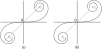
\includegraphics[scale=1]{figures/ch_18/fig_18_25.pdf}
		% \caption[]{}
        \caption[]{Fresnel diffraction pattern from a slit is either a bright (a) or a relatively dark (b) central fringe at both sides of which there are alternating dark and bright fringes symmetrical relative to it.}
		\label{fig:18_25}
	\end{center}
	\vspace{-0.8cm}
\end{figure}

\section{Fraunhofer Diffraction from a Slit}\label{sec:18_5}

Assume that a plane light wave falls on an infinitely long\footnote{In practice, it is sufficient that the length of the slit he many times its width.} slit (\fig{18_26}).
Let us place a converging lens behind the slit and a screen in the focal plane of the lens.
The wave surface of the incident wave, the plane of the slit, and the screen are parallel to one
another.
Since the slit is infinite, the pattern observed in any plane at right angles to the slit will be the same.
It is therefore sufficient to investigate the nature of the pattern in one such plane, for example, in that of \fig{18_26}.
All the quantities introduced in the following, in particular the angle $\varphi$ made by a ray with the optical axis of the lens, relate to this plane.

\begin{figure}[t]
	\begin{center}
		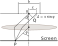
\includegraphics[scale=1]{figures/ch_18/fig_18_26.pdf}
		% \caption[]{}
        \caption[]{A plane light wave hitting on an infinitely long slit. A converging lens is placed behind the slit and a screen in the focal plane of the lens. The wave surface of the incident wave, the plane of the slit, and the screen are parallel to one another.}
		\label{fig:18_26}
	\end{center}
	\vspace{-0.8cm}
\end{figure}

Let us divide the open part of the wave surface into elementary zones of width $\deriv{x}$ parallel to the edges of the slit.
The secondary waves emitted by the zones in the
direction determined by the angle $\varphi$ will gather at point P of the screen.
Each elementary zone will produce the oscillation $\deriv{E}$ at point P.
The lens will gather plane (and not spherical) waves in the focal plane.
Therefore, the factor $1/r$ in \eqn{18_1} for $\deriv{E}$ will be absent for Fraunhofer diffraction.
Limiting ourselves to a consideration of not too great angles $\varphi$, we can assume that the coefficient $K$ in \eqn{18_1} is constant.
Hence, the amplitude of the oscillation produced by a zone at any point of the screen will depend only on the area of the zone.
The area is proportional to the width $\deriv{x}$ of a zone.
Consequently, the amplitude $\deriv{A}$ of the oscillation $\deriv{E}$ produced by a zone of width $\deriv{x}$ at any point of the screen will have the form
\begin{equation*}
	\deriv{A} = C\, \deriv{x},
\end{equation*}

\noindent
where $C$ is a constant.

Let $A_0$ stand for the algebraic sum of the amplitudes of the oscillations produced by all the zones at a point of the screen.
We can find $A_0$ by integrating $\deriv{A}$ over the entire width of the slit $b$:
\begin{equation*}
	A_0 = \int \deriv{A} = \int^{+b/2}_{-b/2} C\, \deriv{x} = C b.
\end{equation*}

\noindent
Hence, $C=A_0/b$ and, therefore,
\begin{equation*}
	\deriv{A} = \frac{A_0}{b}\, \deriv{x}.
\end{equation*}

Now let us find the phase relations between the oscillations $\deriv{E}$.
We shall compare the phases of the oscillations produced at point P by the elementary zones having the coordinates $0$ and $x$ (\fig{18_26}).
The optical paths $0$P and QP are tautochronous (see \fig{16_20}).
Therefore, the phase difference between the oscillations being considered is formed on the path $\Delta$ equal to $x\sin\varphi$.
If the initial phase of the oscillation produced at point P by the elementary zone at the middle of the slit ($\varphi=0$) is assumed to equal zero, then the initial phase of the oscillation produced by the zone with the coordinate $x$ will be
\begin{equation*}
	-2 \pi \frac{\Delta}{\lambda} = - \frac{2\pi}{\lambda} x \sin\varphi,
\end{equation*}

\noindent
where $\lambda$ is the wavelength in the given medium.

Thus, the oscillation produced by the elementary zone with the coordinate $x$ at point P (whose position is determined by the angle $\varphi$) can be written in the form
\begin{equation}\label{eq:18_21}
	\deriv{E_{\varphi}} = \parenthesis{\frac{A_0}{b}\, \deriv{x}}\, \exp\bracket{ i \parenthesis{ \omega t - \frac{2\pi}{\lambda} x \sin\varphi } }
\end{equation}

\noindent
(we have in mind the real part of this expression).

Integrating \eqn{18_21} over the entire width of the slit, we shall find the resultant oscillation produced at point P by the part of the wave surface uncovered by the slit:
\begin{equation*}
	E_{\varphi} = \int^{+b/2}_{-b/2} \parenthesis{ \frac{A_0}{b} }\, \exp\bracket{ i \parenthesis{ \omega t - \frac{2\pi}{\lambda} x \sin\varphi } }\, \deriv{x}.
\end{equation*}

\noindent
Let us put the multipliers not depending on $x$ outside the integral In addition, we shall introduce the symbol
\begin{equation}\label{eq:18_22}
	\gamma = \frac{\pi}{\lambda} \sin\varphi.
\end{equation}

\noindent
As a result, we get
\begin{align*}
	E_{\varphi} &= \frac{A_0}{b} e^{i\omega t} \int^{+b/2}_{-b/2} e^{-2i\gamma x}\, \deriv{x} = \frac{A_0}{b} e^{i\omega t} \parenthesis{ -\frac{1}{2i\gamma} } \left. e^{-2i\gamma x} \right|^{+b/2}_{-b/2}\\
	&= e^{i\omega t} \bracket{ \frac{A_0}{\gamma b} \parenthesis{ -\frac{1}{2i} } \parenthesis{ e^{-i\gamma b} - e^{i\gamma b} } } = e^{i\omega t} \bracket{ \frac{A_0}{\gamma b} \frac{1}{2i} \parenthesis{ e^{i\gamma b} - e^{-i\gamma b} } }.
\end{align*}

The expression in brackets determines the complex amplitude $\hat{A}_{\varphi}$ of the resultant oscillation.
Taking into account that the difference between the exponents divided by $2i$ is $\sin(\gamma b)$ (see Sec. 7.3 of Vol. I), we can write
\begin{equation}\label{eq:18_23}
	\hat{A}_{\varphi} = A_0 \frac{\sin(\gamma b)}{\gamma b} = A_0 \frac{\sin[(\pi b \sin\varphi)/\lambda]}{[(\pi b \sin\varphi)/\lambda]}
\end{equation}

\noindent
[we have introduced the value of $\gamma$ from \eqn{18_22}].

Equation \eqref{eq:18_23} is a real one.
Its magnitude is the usual amplitude of the resultant oscillation:
\begin{equation}\label{eq:18_24}
	A_{\varphi} = \absolute{ A_0 \frac{\sin[(\pi b \sin\varphi)/\lambda]}{[(\pi b \sin\varphi)/\lambda]} }.
\end{equation}

For a point opposite the centre of the lens, $\varphi=0$.
Introduction of this value into \eqn{18_24} gives the value $A_0$ for the amplitude\footnote{We remind our reader that $\lim_{u\to 0}\sin u/u = 1$ (at small values of $u$ we may assume that sin $\sin u \approx u$).}.
This result can be obtained in a simpler way. When $\varphi=0$, the oscillations from all the elementary zones arrive at point P in the same phase.
Therefore, the amplitude of the resultant oscillation equals the algebraic sum of the amplitudes of the oscillations being added.

At values of $\varphi$ satisfying the condition $(\pi b\sin\varphi)/\lambda=\pm k\pi$, \ie, when
\begin{equation}\label{eq:18_25}
	b \sin\varphi = \pm k \lambda \quad (k = 1, 2, 3, \ldots),
\end{equation}

\noindent
the amplitude $A_{\varphi}$ vanishes.
Thus, condition \eqref{eq:18_25} determines the positions of the minima of intensity.
We must note that $b\sin\varphi$ is the path difference $\Delta$ of the rays travelling to point P from the edges of the slit (see \fig{18_26}).

It is easy to obtain condition \eqref{eq:18_25} from the following considerations.
If the path difference $\Delta$ from the edges of the slit is $\pm k\lambda$, the uncovered part of the wave surface can be divided into $2k$ zones equal in width, and the path difference from the edges of each zone will be $\lambda/2$ (see \fig{18_27} for $k=2$).
The oscillations from each pair of adjacent zones mutually destroy each other, so that the resultant
amplitude vanishes.
If the path difference $\Delta$ for point P is $+(k+1/2)\lambda$, the number of zones will be odd, the action of one of them will not be compensated, and a maximum of intensity is observed.

The intensity of light is proportional to the square of the amplitude.
Hence, in accordance with \eqn{18_24},
\begin{equation}\label{eq:18_26}
	I_{\varphi} = I_0 \frac{\sin^2[(\pi b \sin\varphi)\lambda]}{[(\pi b \sin\varphi)\lambda]^2},
\end{equation}

\noindent
where $I_0$ is the intensity at the middle of the diffraction pattern (opposite the centre of the lens), and $I_{\varphi}$ is the intensity at the point whose position is determined by the given value of $\varphi$.

We find from \eqn{18_26} that $I_{-\varphi}=I_{\varphi}$.
This signifies that the diffraction pattern is symmetrical relative to the centre of the lens.
We must note that when the slit is displaced parallel to the screen (along the $x$-axis in \fig{18_26}), the diffraction pattern observed on the screen remains stationary (its middle is  opposite the centre of the lens).
Conversely, displacement of the lens with the slit stationary is attended by the same displacement of the pattern on the screen.

\begin{figure}[t]
	\begin{minipage}[t]{0.48\linewidth}
		\begin{center}
			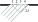
\includegraphics[scale=1]{figures/ch_18/fig_18_27.pdf}
			% \caption[]{}
            \caption[]{Destruction and construction of oscillations for a path difference $\Delta$ from the edges of the slit equal to $\pm k\lambda$ and to $+(k+1/2)\lambda$, respectively, with $k=2$.}
			\label{fig:18_27}
		\end{center}
	\end{minipage}
	\hfill{ }%space{-0.05cm}
	\begin{minipage}[t]{0.48\linewidth}
		\begin{center}
			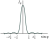
\includegraphics[scale=1]{figures/ch_18/fig_18_28.pdf}
            % \caption[]{}
			\caption[]{Graph of function \eqref{eq:18_26}. The number of intensity minima is determined by the ratio of the width of a slit $b$ to the wavelength $\lambda$.}
			\label{fig:18_28}
		\end{center}
	\end{minipage}
\vspace{-0.4cm}
\end{figure}

A graph of function \eqref{eq:18_26} is depicted in \fig{18_28}.
The values of $\sin\varphi$ are laid off along the axis of abscissas, and the intensity $I_{\varphi}$
along the axis of ordinates.
The number of intensity minima is determined by the ratio of the width of a slit $b$ to the wavelength $\lambda$.
It can be seen from condition \eqref{eq:18_25} that $\sin\varphi=\pm k\lambda/b$.
The magnitude of $\sin\varphi$ cannot exceed unity.
Hence, $k\lambda/b\geqslant 1$, whence
\begin{equation}\label{eq:18_27}
	k \geqslant \frac{b}{\lambda}.
\end{equation}

\noindent
At a slit width less than a wavelength, minima do not appear at all.
In this case, the intensity of the light monotonously diminishes from the middle of the pattern toward its edges.

The values of the angle $\varphi$ obtained from the condition $b\sin\varphi=\pm\lambda$ correspond to the edges of the central maximum.
These values are $\pm\arcsin(\lambda/b)$.
Consequently, the angular width of the central maximum is
\begin{equation}\label{eq:18_28}
	\delta\varphi = 2 \arcsin\parenthesis{\frac{\lambda}{b}}.
\end{equation}

\noindent
When $b\gg\lambda$, the value of $\sin(\lambda/b)$ can be assumed equal to $\lambda/b$.
The equation for the angular width of the central maximum is thus simplified as follows:
\begin{equation}\label{eq:18_29}
	\delta\varphi = \frac{2 \lambda}{\varphi}.
\end{equation}

\begin{figure}[t]
	\begin{center}
		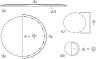
\includegraphics[scale=1]{figures/ch_18/fig_18_29.pdf}
		% \caption[]{}
        \caption[]{Solution of the problem on the Fraunhofer diffraction from a slit by the method of graphical summation of the amplitudes. The open part of the wave surface is divided into very narrow zones of an identical width. The oscillation produced by each of these zones has the same amplitude $\Delta{A}$ and lags in phase behind the preceding oscillation by the same value $\delta$ that depends on the angle $\varphi$ determining the direction to the point of observation P. (a) Vector diagram with $\varphi=0, \delta=0$. (b) When $\Delta=b\sin\varphi= \lambda/2$, the vectors $\Delta{\vec{A}}$ form a semicircle of length $A_0$. (c) When $\Delta=b\sin\varphi=\lambda$, the vectors $\Delta{\vec{A}}$ arrange themselves along a semicircle of length $A_0$, but with phase difference equal o $2\pi$. (d) Constructing sequentially the vectors $\Delta{\vec{A}}$,  when $\Delta=b\sin\varphi=3\lambda/2$, we travel one and a half times around a circle of diameter $A_1=2A_0/3\pi$, which is the amplitude of the first maximum.}
		\label{fig:18_29}
	\end{center}
	\vspace{-0.8cm}
\end{figure}

Let us solve the problem on the Fraunhofer diffraction from a slit by the method of graphical summation of the amplitudes.
We divide the open part of the wave surface into very narrow zones of an identical width.
The oscillation produced by each of these zones has the same amplitude $\Delta{A}$ and lags in phase behind the preceding oscillation by the same value $\delta$ that depends on the angle $\varphi$ determining the direction to the point of observation P.
When $\varphi=0$, the phase difference $\delta$ vanishes, and the vector diagram has the form shown in \fig{18_29}a.
The amplitude of the resultant oscillation $A_0$ equals the algebraic sum of the amplitudes of the oscillations being added.
When $\Delta=b\sin\varphi=\lambda/2$, the oscillations from edges of the slit are in counterphase.
Accordingly, the vectors $\Delta{\vec{A}}$ arrange themselves along a semicircle of length $A_0$ (\fig{18_29}b).
Hence, the resultant amplitude is $2A_0/\pi$.
When $\Delta=b\sin\varphi=\lambda$, the oscillations from the edges of the slit differ in phase by $2\pi$.
The corresponding vector diagram is shown in \fig{18_29}c.
The vectors $\Delta{\vec{A}}$ arrange themselves along a circle of length $A_0$.
The resultant amplitude is zero---the first minimum is obtained.
The first maximum is obtained at $\Delta=b\sin\varphi=3\lambda/2$.
In this case, the oscillations from the edges
of the slit differ in phase by $3\pi$.
Constructing sequentially the vectors $\Delta{\vec{A}}$, we travel one and a half times around a circle of diameter $A_1=2A_0/3\pi$ (\fig{18_29}d).
It is exactly the diameter of this circle that is the amplitude of the first maximum.
Thus, the intensity of the first maximum is $I_1= (2/3\pi)^2I_0\approx 0.045 I_0$.
We can find the relative intensity of the other maxima in a similar way.
As a result, we get the following proportion:
\begin{equation}\label{eq:18_30}
	I_0 : I_1 : I_2 : I_3 : \ldots = \parenthesis{\frac{2}{3\pi}}^2 : \parenthesis{\frac{2}{5\pi}}^2 : \parenthesis{\frac{2}{7\pi}}^2 : \ldots.
\end{equation}

\noindent
Thus, the central maximum considerably exceeds the remaining maxima in intensity; the main fraction of the light flux passing through the slit is concentrated in it.

When the width of the slit is very small in comparison with the distance from it to the screen, the rays travelling to point P from the edges of the slit will be virtually parallel even in the absence of a lens between the slit and the screen.
Consequently, when a plane wave falls on a slit, Fraunhofer diffraction will be observed.
All the equations obtained above will hold; by $\varphi$ in them one should understand the angle between the direction from any edge of the slit to point P and a normal to the plane of the slit.

Let us establish a quantitative criterion permitting us to determine the kind of diffraction that will occur in each particular case.
We shall find the path difference of the rays from the edges of the slit to point P (\fig{18_30}).
We apply the cosine law to the triangle with the legs $r$, $r+\Delta$, and $b$:
\begin{equation*}
	(r+\Delta)^2 = r^2 + b^2 - 2rb \cos\parenthesis{\frac{\pi}{2} + \varphi}.
\end{equation*}

\begin{figure}[t]
	\begin{center}
		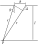
\includegraphics[scale=1]{figures/ch_18/fig_18_30.pdf}
		% \caption[]{}
        \caption[]{Path difference of the rays from the edges of the slit to point P, to determine the kind of diffraction that will occur in each particular case.}
		\label{fig:18_30}
	\end{center}
	\vspace{-0.8cm}
\end{figure}

Simple transformations yield
\begin{equation}\label{eq:18_31}
	2r\Delta + \Delta^2 = b^2 + 2rb \sin\varphi.
\end{equation}

\noindent
We are interested in the case when the rays travelling from the edges of the slit to point P are almost parallel.
When this condition is observed, $\Delta^2\ll r\Delta$, and we can therefore ignore the addend $\Delta^2$ in \eqn{18_31}.
In this approximation
\begin{equation}\label{eq:18_32}
	\Delta = \frac{b^2}{2r} + b \sin\varphi.
\end{equation}

\noindent
In the limit at $r\to\infty$, we get a value of the path difference $\Delta_{\infty}=b \sin\varphi$ that coincides with the expression in \eqn{18_25}.

At finite $r$'s, the nature of the diffraction pattern will be determined by the relation between the difference $\Delta-\Delta_{\infty}$ and the wavelength $\lambda$.
If
\begin{equation}\label{eq:18_33}
	\Delta-\Delta_{\infty} = \ll \lambda,
\end{equation}

\noindent
the diffraction pattern will be virtually the same as in Fraunhofer diffraction.
At $\Delta-\Delta_{\infty}$ comparable with $\lambda$ (\ie, $\Delta-\Delta_{\infty}\sim \lambda$), Fresnel diffraction will take place.
It follows from \eqn{18_32} that
\begin{equation*}
	\Delta-\Delta_{\infty} = \frac{b^2}{2r} \sim \frac{b^2}{l}
\end{equation*}

\noindent
(here, $l$ is the distance from the slit to the screen).
Introduction of this expression into inequality \eqref{eq:18_33} gives the condition $(b^2/l)\ll\lambda$ or
\begin{equation}\label{eq:18_34}
	\frac{b^2}{l\lambda} \ll 1.
\end{equation}

\noindent
Thus, the nature of diffraction depends on the value of the dimensionless parameter
\vspace{-12pt}
\begin{equation}\label{eq:18_35}
	\frac{b^2}{l\lambda}.
\end{equation}

If this parameter is much smaller than unity, Fraunhofer diffraction is observed, if it is of the order of unity, Fresnel diffraction is observed, and, finally, if this parameter is much greater than unity, the approximation of geometrical optics is applicable.
For convenience of comparison, let us write what has been said above in the following form:
\begin{equation}\label{eq:18_36}
	\frac{b^2}{l\lambda}
	\begin{cases}
		\ll 1 & \Rightarrow \text{ Fraunhofer diffraction,}\\
		\sim 1 & \Rightarrow \text{ Fresnel diffraction,}\\
		\gg 1 & \Rightarrow \text{ geometrical optics.}\\
	\end{cases}
\end{equation}

Parameter \eqref{eq:18_35} can be given a visual interpretation.
Let us take point P opposite the middle of a slit (\fig{18_31}).
For this point, the number $m$ of Fresnel zones opened by the slit is determined by the expression
\begin{equation*}
	\parenthesis{l + m \frac{\lambda}{2}}^2 = l^2 + \parenthesis{\frac{b}{2}}^2.
\end{equation*}

\begin{figure}[t]
	\begin{center}
		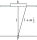
\includegraphics[scale=0.95]{figures/ch_18/fig_18_31.pdf}
		% \caption[]{}
        \caption[]{Diagram to make a visual interpretation of the parameter \eqref{eq:18_35}. $m$ is the number of Fresnel zone, $\lambda$ the wavelength, $b$ is the width of the slit and $l$ the distance from the middle of the slit to the point P.}
		\label{fig:18_31}
	\end{center}
	\vspace{-0.8cm}
\end{figure}

Opening the parentheses and discarding the addend proportional to $\lambda^2$, we get\footnote{We must note that the number of open zones will be larger for points greatly displaced to the region of the geometrical shadow.}
\vspace{-12pt}
\begin{equation}\label{eq:18_37}
	m = \frac{b^2}{4l\lambda} \sim \frac{b^2}{l\lambda}.
\end{equation}

\noindent
Thus, parameter \eqref{eq:18_35} is directly associated with the number of uncovered Fresnel zones (for a point opposite the middle of the slit).

If a slit opens a small fraction of the central Fresnel zone ($m\ll 1$), Fraunhofer diffraction is observed.
The distribution of the intensity in this case is shown by the curve depicted in \fig{18_28}.
If a slit uncovers a small number of Fresnel zones ($m\sim 1$), an image of the slit surrounded along its edges by clearly visible bright and dark fringes will be obtained on the screen.
Finally, when a slit opens a large number of Fresnel zones ($m\gg 1$), a uniformly illuminated
image of the slit is obtained on the screen.
Only at the boundaries of the geometrical shadow are there very narrow alternating brighter and darker fringes virtually indistinguishable by the eye.

Let us see how the pattern changes when the screen is moved away from the slit.
When the screen is near the slit ($m\gg 1$), the image corresponds to the laws of geometrical optics.
Upon increasing the distance, we first obtain a Fresnel diffraction pattern which then transforms into a Fraunhofer pattern.
The same sequence of changes is observed when we reduce the width of the slit $b$ without changing
the distance $l$.

It is clear from what has been said above that the value of the parameter \eqref{eq:18_35} is the criterion of the applicability of geometrical optics (it must be much greater than unity) instead of the smallness of the wavelength in comparison with the characteristic dimension of the barrier (for example, the width of the slit).
Assume, for instance, that both ratios $b/\lambda$ and $l/b$ equal $100$.
In this case, $\lambda\ll b$, but $b^2/(l\lambda)=1$, and, therefore, a distinctly expressed Fresnel diffraction pattern will be observed.

\section{Diffraction Grating}\label{sec:18_6}

A diffraction grating is a collection of a large number of identical equispaced slits (\fig{18_32}).
The distance $d$ between the centres of adjacent slits is called the \textbf{period} of the grating.

\begin{figure}[t]
	\begin{center}
		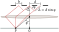
\includegraphics[scale=0.95]{figures/ch_18/fig_18_32.pdf}
		% \caption[]{}
        \caption[]{Scheme of a diffraction grating with period $d$ and slit width $b$. A converging lens is parallel to it focus a normal incident light and a screen in the focal plane of the lens serves to check the diffraction pattern similar to that of \fig{18_28}.}
		\label{fig:18_32}
	\end{center}
	\vspace{-0.9cm}
\end{figure}

Let us place a converging lens parallel to a grating and put a screen in the focal plane of the lens.
We shall determine the nature of the diffraction pattern obtained on the screen when a plane light wave falls on the grating (we shall consider for
simplicity's sake that the wave falls normally on the grating).
Each slit produces a pattern on the screen that is
described by the curve depicted in \fig{18_28}.
The patterns from all the slits will be at the same place on the screen (regardless of the position of the slit, the central maximum is opposite the centre of the lens).
If the oscillations arriving at point P from different slits were incoherent, the resultant pattern produced by $N$ slits would differ from the pattern produced by a single slit only in that all the intensities would grow $N$ times.
The oscillations from different slits are coherent to a greater or smaller extent, however.
The resultant intensity will therefore differ from $NI_{\varphi}$ [$I_{\varphi}$ is the intensity produced by one slit; see \eqn{18_26}].

We shall assume in the following that the coherence radius of the incident wave is much greater than the length of the grating so that the oscillations from all the slits can be considered coherent relative to one another.
In this case, the resultant oscillation at point P
whose position is determined by the angle $\varphi$ is the sum of $N$ oscillations having the same amplitude $A_{\varphi}$ shifted relative to one another in phase by the same amount $\delta$.
According to \eqn{17_47}, the intensity in these conditions is
\begin{equation}\label{eq:18_38}
	\ab{I}{gr} = I_{\varphi} \frac{\sin^2(N\delta/2)}{\sin^2(\delta/2)}
\end{equation}

\noindent
(here $I_{\varphi}$ plays the part of $I_0$).

A glance at \fig{18_32} shows that the path difference from adjacent slits is $\delta=d \sin\varphi$.
Hence, the phase difference is
\begin{equation}\label{eq:18_39}
	\delta = 2\pi \frac{\Delta}{\lambda} = \frac{2\pi}{\lambda} d \sin\varphi,
\end{equation}

\noindent
where $\lambda$ is the wavelength in the given medium.

Introducing into \eqn{18_38} \eqns{18_26}{18_39} for $I_{\varphi}$ and $\delta$, respectively, we get
\begin{equation}\label{eq:18_40}
	\ab{I}{gr} = I_0 \frac{\sin^2(\pi b \sin\varphi /\lambda)}{(\pi b \sin\varphi /\lambda)^2} \frac{\sin^2(N\pi d \sin\varphi /\lambda)}{sin^2(\pi d \sin\varphi /\lambda)}
\end{equation}

\noindent
($I_0$ is the intensity produced by one slit opposite the centre of the lens).

The first multiplier of $I_0$ in \eqn{18_40} vanishes condition \eqref{eq:18_25} is observed, \ie,
\begin{equation*}
	b \sin\varphi = \pm k \lambda \quad (k = 1, 2, 3, \ldots).
\end{equation*}

At these points, the intensity produced by each slit individually equals zero.

The second multiplier of $I_0$ in \eqn{18_40} acquires the value $N^2$ for points satisfying the condition
\begin{equation}\label{eq:18_41}
	d \sin\varphi = \pm m \lambda \quad (m = 0, 1, 2, \ldots)
\end{equation}

\noindent
[see \eqn{17_49}].
For the directions determined by this condition, the oscillations from individual slits mutually amplify one another.
As a result, the amplitude of the oscillations at the corresponding point of the screen is
\begin{equation}\label{eq:18_42}
	\ab{A}{max} = N A_{\varphi}
\end{equation}

\noindent
($A_{\varphi}$ is the amplitude of the oscillation emitted by one slit at the angle $\varphi$).

Condition \eqref{eq:18_41} determines the positions of the intensity maxima called the \textbf{principal} ones.
The number $m$ gives the order of the principal maximum.
There is only one zero-order maximum, and there are two each of the maxima of the $1$st, $2$nd, etc. orders.

Squaring \eqn{18_42}, we find that the intensity of the principal maxima $\ab{I}{max}$ is $N^2$ times greater than the intensity $I_{\varphi}$, produced in the direction $\varphi$ by a single slit:
\begin{equation}\label{eq:18_43}
	\ab{I}{max} = N^2 I_{\varphi}.
\end{equation}

Apart from the minima determined by condition \eqref{eq:18_25}, there are $N-1$ additional minima in each interval between adjacent principal maxima.
These minima appear in the directions for which the oscillations from individual slits mutually destroy one another.
In accordance with \eqn{17_50}, the directions of the additional minima are determined by the condition
\begin{equation}\label{eq:18_44}
	d \sin\varphi = \pm \frac{k'}{N} \lambda (k'=1,2,\ldots,N-1,N+1,\ldots,2N-1,2N+1,\ldots).
\end{equation}

\noindent
In \eqn{18_44}, $k'$ takes on all integral values except for $0, N, 2N, \ldots$, \ie, except for those at which \eqn{18_44} transforms into
\eqn{18_41}.

It is easy to obtain condition \eqref{eq:18_44} by the method of graphical addition of oscillations.
The oscillations from the individual slits are depicted by vectors of the same length.
According to \eqn{18_44}, each of the following vectors is turned relative to the preceding one by the same angle
\begin{equation*}
	\delta = \frac{2\pi}{\lambda} d\sin\varphi = \frac{2\pi}{\lambda} k'.
\end{equation*}

\noindent
Therefore, when $k'$ is not an integral multiple of $N$, we put the tip of the following vector against the tail of the preceding one and obtain a closed broken line that completes $k'$ (when $k'<N/2$) or $N-k'$ (when $k'>N/2$) revolutions before the tail of the $N$-th vector contacts the tip of the first one.
The resultant amplitude accordingly equals zero. The above is explained in \fig{18_33} that shows the sum of the vectors for $N=9$ and for the values of $k'$ equal to $1, 2$, and $N-1=8$.

\begin{figure}[t]
	\begin{center}
		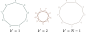
\includegraphics[scale=0.95]{figures/ch_18/fig_18_33.pdf}
		% \caption[]{}
        \caption[]{Method of graphical addition of oscillations to arrive at \eqn{18_44}. Sum of the vectors for $N = 9$ and for the values of $k'$ equal to $1, 2$, and $N-1= 8$.}
		\label{fig:18_33}
	\end{center}
	\vspace{-0.7cm}
\end{figure}

Between the additional minima, there are weak secondary maxima.
The number of such maxima falling to an interval between adjacent principal maxima is $N-2$.
We showed in \sect{17_6} that the intensity of the secondary maxima does not exceed $1/22$nd of that of the closest principal maximum.

\begin{figure}[t]
	\begin{center}
		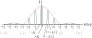
\includegraphics[scale=1.1]{figures/ch_18/fig_18_34.pdf}
		% \caption[]{}
        \caption[]{Graph of \eqn{18_40} for $N=4$ and $d/b=3$. The dash curve shows the intensity produced by one slit multiplied by $N^2$ [\eqn{18_43}].}
		\label{fig:18_34}
	\end{center}
	\vspace{-0.8cm}
\end{figure}

Figure \ref{fig:18_34} shows a graph of function \eqref{eq:18_40} for $N=4$ and $d/b=3$.
The dash curve passing through the peaks of the principal maxima shows the intensity produced by one slit multiplied by $N^2$ [see \eqn{18_43}].
At the ratio of the grating period to the slit width used in the figure ($d/b=3$), the principal maxima of the third, sixth, etc. orders fall to the minima of intensity from one slit, owing to which these maxima vanish.
In general, it can be seen from \eqns{18_25}{18_41} that the principal maximum of the $m$-th order falls to the $k$-th minimum from one slit if the equation $m/d = k/b$ or $m/k = d/b$ is satisfied.
This is possible if $d/b$ equals the ratio of two integers $r$ and $s$ (the ease when these integers are not great is of practical interest).
Here, the principal maximum of the $r$-th order will be superposed on the $s$-th minimum from one slit, the maximum of the $2r$-th order will be superposed on the $2s$-th minimum, etc.
As a result, the maxima of orders $r$, $2r$, $3r$, etc. will be absent.

The number of principal maxima observed is determined by the ratio of the period of the grating $d$ to the wavelength $\lambda$.
The magnitude of $\sin\varphi$ cannot exceed unity.
It therefore follows from \eqn{18_41} that
\begin{equation}\label{eq:18_45}
	m \leqslant \frac{d}{\lambda}.
\end{equation}

Let us determine the angular width of the central (zero) maximum.
The position of the additional minima closest to it is determined by the condition $d\sin\varphi= \pm\lambda N$ [see \eqn{18_44}].
Hence, values of $\varphi$ equal to $\pm\arcsin(\lambda/Nd)$ correspond to these minima.
We thus obtain the following expression for the angular width of the central maximum:
\begin{equation}\label{eq:18_46}
	\delta\varphi_0 = 2 \arcsin\parenthesis{\frac{\lambda}{Nd}} \approx \frac{2\lambda}{Nd}
\end{equation}

\noindent
(we have taken advantage of the circumstance that$\lambda/ND \ll 1$).

The position of the additional minima closest to the principal maximum of the $m$-th order is determined by the condition $d\sin\varphi = (m \pm 1/N)\lambda$.
Hence, for the angular width of the $m$-th maximum, we get the expression
\begin{equation*}
	\delta\varphi_m = 2 \arcsin\parenthesis{m + \frac{1}{N}} \frac{\lambda}{d} - \arcsin\parenthesis{m - \frac{1}{N}} \frac{\lambda}{d}.
\end{equation*}

\noindent
Introducing the notation $m\lambda/d=x$ and $\lambda/Nd=\Delta{x}$, we can write this equation in the form
\begin{equation}\label{eq:18_47}
	\delta\varphi_m = \arcsin(x + \Delta{x}) - \arcsin(x - \Delta{x}).
\end{equation}

\noindent
With a great number of slits, the value of $\Delta{x}=\lambda/Nd$ will be very small.
We can therefore assume that $\arcsin(x\pm\Delta{x})\sim\arcsin x \pm (\arcsin x)' \Delta{x}$.
The introduction of these values into \eqn{18_47}
leads to the approximate expression
\begin{equation}\label{eq:18_48}
	\delta\varphi_m = 2 (\arcsin x)' \Delta{x} = \frac{2 \Delta{x}}{\sqrt{1-x^2}} = \frac{1}{\sqrt{1 - m^2(\lambda/d^2)^2}} \frac{\lambda}{Nd}.
\end{equation}

\noindent
When $m=0$, this expression transforms into \eqn{18_46}.

The product $Nd$ gives the length of the diffraction grating.
Consequently, the angular width of the principal maxima is inversely proportional to the length of the grating.
The width $\delta{\varphi_m}$ grows with an increase in the order $m$ of a maximum.

The position of the principal maxima depends on the wavelength $\lambda$.
Therefore, when white light is passed through a grating, all the maxima except for the central one will expand into a spectrum whose violet end faces the centre of the diffraction pattern, and
whose red end faces outward.
Thus, a diffraction grating is a spectral instrument.
We must note that whereas a glass prism deflects violet rays the greatest, a diffraction grating, on the contrary, deflects red rays to a greater extent.

Figure \ref{fig:18_35} shows schematically the spectra of different orders produced by a grating when white light is passed through it.
At the centre is a narrow zero-order maximum; only its edges are coloured [according to expression \eqref{eq:18_46}, $\delta{\varphi_0}$ depends on $\lambda$].
At both sides of the central maximum are two first-order spectra, then two second-order spectra, etc.
The positions of the red end of the $m$-th order spectrum and the violet end of the $(m+1)$-th order one are determined by the relations
\begin{equation*}
	\sin\ab{\varphi}{r} = m \frac{0.76}{d},\quad \sin\ab{\varphi}{v} = (m+1) \frac{0.40}{d},
\end{equation*}

\noindent
where $d$ has been taken in micrometres.
When the condition is observed that
\begin{equation*}
	0.76 m > 0.40 (m+1),
\end{equation*}

\noindent
the spectra of the $m$-th and $(m+1)$-th orders partly overlap.
The inequality gives $m>10/9$.
Hence, partial overlapping begins from the spectra of the second and third orders (see \fig{18_35}, in which for illustration the spectra of different orders are displaced relative to one another vertically).

The main characteristics of a spectral instrument are its \textbf{dispersion} and \textbf{resolving power}.
The dispersion determines the angular or linear distance between two spectral lines differing in wavelength by one unit (for example by \SI{1}{\angstrom}).
The resolving power determines the minimum difference between wavelengths $\delta{\lambda}$ at which the two lines corresponding to them are perceived separately in the spectrum.

The \textbf{angular dispersion} is defined as the quantity
\begin{equation}\label{eq:18_49}
	D = \frac{\delta{\varphi}}{\delta{\lambda}},
\end{equation}

\noindent
where $\delta{\varphi}$ is the angular distance between spectral lines differing in wavelength by $\delta{\lambda}$.

To find the angular dispersion of a diffraction grating, let us differentiate condition \eqref{eq:18_41} for the principal maximum at the
left with respect to $\varphi$ and at the right with respect to $\lambda$.
Omitting the minus sign, we get
\begin{equation*}
	(d\cos\varphi) \delta{\varphi} = m\, \delta{\lambda},
\end{equation*}

\noindent
whence
\begin{equation}\label{eq:18_50}
	D = \frac{\delta{\varphi}}{\delta{\lambda}} = \frac{m}{d\cos\varphi}.
\end{equation}

\noindent
Within the range of small angles; $\cos\varphi\approx 1$.
We can therefore assume that
\begin{equation}\label{eq:18_51}
	D \approx \frac{m}{d}.
\end{equation}

\noindent
It can be seen from expression \eqref{eq:18_51} that the angular dispersion is inversely proportional to the grating period $d$.
The higher the order $m$ of a spectrum, the greater is the dispersion.

\begin{figure}[t]
	\begin{center}
		
\includegraphics[scale=1]{figures/ch_18/fig_18_35.pdf}
		% \caption[]{}
        \caption[]{Scheme of the spectra of different orders produced by a grating when white light is passed through it. At the centre there is a narrow zero-order maximum and only its edges are coloured [\eqn{18_46}]. At both sides of the central maximum are two first-order spectra, then two second-order spectra, etc.}
		\label{fig:18_35}
	\end{center}
	\vspace{-0.8cm}
\end{figure}

\textbf{Linear dispersion} is defined as the quantity
\begin{equation}\label{eq:18_52}
	\ab{D}{lin} = \frac{\delta{l}}{\delta{\lambda}},
\end{equation}

\noindent
where $\delta{l}$ is the linear distance on a screen or photographic plate between spectral lines differing in wavelength by $\delta{\lambda}$.
A glance at \fig{18_36} shows that for small values of the angle $\varphi$ we can assume that $\delta{l}\approx f'\delta{\varphi}$, where $f'$ is the focal length of the lens gathering the diffracted rays on a screen.
Consequently, the linear dispersion is associated with the angular dispersion $D$ by the relation
\begin{equation*}
	\ab{D}{lin} = f' D.
\end{equation*}

\noindent
Taking expression \eqref{eq:18_51} into consideration, we get the following equation for the linear dispersion of a diffraction grating (with small $\varphi$'s):
\begin{equation}\label{eq:18_53}
	\ab{D}{lin} = f' \frac{m}{d}.
\end{equation}

The resolving power of a spectral instrument is defined as the dimensionless quantity
\begin{equation}\label{eq:18_54}
	R = \frac{\lambda}{\delta{\lambda}},
\end{equation}

\noindent
where $\delta{\lambda}$ is the minimum difference between the wavelengths of two spectral lines at which these lines are perceived separately.

\begin{figure}[t]
	\begin{minipage}[t]{0.48\linewidth}
		\begin{center}
			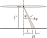
\includegraphics[scale=0.95]{figures/ch_18/fig_18_36.pdf}
			% \caption[]{}
            \caption[]{For small values of the angle $\varphi$ we can assume that $\delta{l}\approx f'\delta{\varphi}$, where $f'$ is the focal length of the lens gathering the diffracted rays on a screen.}
			\label{fig:18_36}
		\end{center}
	\end{minipage}
	\hfill{ }%space{-0.05cm}
	\begin{minipage}[t]{0.48\linewidth}
		\begin{center}
			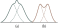
\includegraphics[scale=0.95]{figures/ch_18/fig_18_37.pdf}
            % \caption[]{}
			\caption[]{Resultant intensity (solid curves) observed in the superposition of two close maxima (the dash curves).
			(a) Both maxima are perceived as a single one. (b) There is a minimum between the maxima.}
			\label{fig:18_37}
		\end{center}
	\end{minipage}
\vspace{-0.4cm}
\end{figure}

The possibility of resolving (\ie, perceiving separately) two close spectral lines depends not only on the distance between them (that is determined by the dispersion of the instrument), but also on the width of the spectral maximum.
Figure \ref{fig:18_37} shows the resultant intensity (solid curves) observed in the superposition of two close maxima (the dash curves).
In case (a), both maxima are perceived as a single one.
In case (b), there is a minimum between the maxima.
\textit{Two close maxima are perceived by the eye separately if the intensity in the interval between them is not over $80\%$ of the intensity
of a maximum}.
According to the criterion proposed by the British physicist John Rayleigh (1842-1919), such a ratio of the intensities occurs if the middle of one maximum coincides with the edge of another one (\fig{18_37}b).
Such a mutual arrangement of the maxima is obtained at a definite (for the given instrument) value of $\delta{\lambda}$.

Let us find the resolving power of a diffraction grating.
The position of the middle of the $m$-th maximum for the wavelength $\lambda+\delta{\lambda}$ is riei;ermined by the condition
\begin{equation*}
	d \sin\ab{\varphi}{max} = m (\lambda + \delta{\lambda}).
\end{equation*}

\noindent
The edges of the $m$-th maximum for the wavelength $\lambda$ are at angles complying with the condition
\begin{equation*}
	d \sin\ab{\varphi}{min} = \parenthesis{m \pm \frac{1}{N}} \lambda.
\end{equation*}

\noindent
The middle of the maximum for the wavelength $\lambda + \delta{\lambda}$ coincides with the edge of the maximum for the wavelength $\lambda$ if
\begin{equation*}
	m (\lambda + \delta{\lambda}) = \parenthesis{m \pm \frac{1}{N}} \lambda,
\end{equation*}

\noindent
whence
\begin{equation*}
	m \delta{\lambda} = \frac{\lambda}{N}.
\end{equation*}

\noindent
Solving this equation relative to $\lambda/\delta{\lambda}$, we get an expression for the
resolving power:
\vspace{-12pt}
\begin{equation}\label{eq:18_55}
	R = mN.
\end{equation}

\noindent
Thus, the resolving power of a diffraction grating is proportional to the order $m$ of the spectrum and the number of slits $N$.

Figure \ref{fig:18_38} compares the diffraction patterns obtained for two spectral lines with the aid of gratings differing in the values of the dispersion $D$ and the resolving power $R$.
Gratings I and II have the same resolving power (they have the same number of slits $N$), but a different dispersion (in grating I, the period $d$ is double and the dispersion $D$ is half of the respective quantities of grating II).
Gratings II and III have the same dispersion (they have the same $d$'s), but a different resolving power (the number of slits $N$ and the resolving power $R$ of grating II are double the respective quantities of grating III).

\begin{figure}[t]
	\begin{center}
		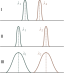
\includegraphics[scale=1.0]{figures/ch_18/fig_18_38.pdf}
		% \caption[]{}
        \caption[]{Comparison of diffraction patterns obtained for two spectral lines with the aid of gratings differing in the values of the dispersion $D$ and the resolving power $R$. Gratings I and II have the same resolving power, but in grating I the period is double and dispersion $D$ is half of that in grating II. Gratings II and III have the same dispersion, but the resolving power of grating II doubles that of grating IIII.}
		\label{fig:18_38}
	\end{center}
	\vspace{-0.8cm}
\end{figure}

Transmission and reflecting diffraction gratings are in use.
Transmission gratings are made from glass or quartz plates on whose surface a special machine using a diamond cutter makes a number of parallel lines.
The spaces between these lines are the slits.

Reflecting gratings are applied with the aid of a diamond cutter on the surface of a metal mirror.
Light falls on a reflecting grating at an acute angle.
A grating of period $d$ functions in the same way
as a transmission grating with the period $d\cos\theta$, where $\theta$ is the angle of incidence of the light, would function with the light falling normally. This makes it possible to observe a spectrum when light is reflected, for example, from a gramophone record having only
a few lines (grooves) per millimetre if it is placed so that the angle of incidence is close to $\pi/2$.
The American physicist Henry Row land (1848-1901) invented a concave reflecting grating which focuses the diffraction spectra by itself (without a lens).

The best gratings have up to $1200$ lines per mm ($d\approx\SI{0.8}{\micro\metre}$).
It can be seen from \eqn{18_45} that no second-order spectra are observed in visible light with such a period.
The total number of lines in such gratings reaches $200000$ (they are about \SI{200}{\milli\metre} long).
With a focal length of the instrument $f'=\SI{2}{\metre}$, the length of the visible first-order spectrum in this case is over \SI{700}{\milli\metre}.

\section{Diffraction of X-Rays}\label{sec:18_7}

Let us place two diffraction gratings one after the other so that their lines are mutually perpendicular.
The first grating (whose lines, say, are vertical) will produce a number of maxima in the horizontal direction.
Their positions are determined by the condition
\begin{equation}\label{eq:18_56}
	d_1 \sin\varphi_1 = \pm m_1 \lambda \quad (m_1=0,1,2\ldots).
\end{equation}

\noindent
The second grating (with horizontal lines) will divide each of the beams formed in this way into vertically arranged maxima whose positions are determined by the condition
\begin{equation}\label{eq:18_57}
	d_2 \sin\varphi_2 = \pm m_2 \lambda \quad (m_2=0,1,2\ldots).
\end{equation}

\noindent
As a result, the diffraction pattern will have the form of regularly arranged spots, with two integral indices $m_1$ and $m_2$ corresponding to each of them (\fig{18_39}).

An identical diffraction pattern is obtained if instead of two separate gratings we take one transparent plate with two systems of mutually perpendicular lines applied on it.
Such a plate is a two-dimensional periodic structure (a conventional grating is a one-dimensional structure).
Having measured the angles $\varphi_1$ and $\varphi_2$  determining the positions of the maxima and knowing the wavelength $\lambda$, we can use \eqns{18_56}{18_57} to find the periods of the structure $d_1$ and $d_2$.
If the directions in which a structure is periodic (for example, directions at right angles to the grating lines) make the angle a differing from $\pi/2$, the diffraction maxima will be at the apices of parallelograms instead of at the apices of rectangles (as in \fig{18_39}).
In this case, the diffraction pattern can be used
to determine not only the periods $d_1$ and $d_2$, but also the angle $\alpha$.

\begin{figure}[t]
	\begin{minipage}[t]{0.48\linewidth}
		\begin{center}
			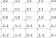
\includegraphics[scale=1]{figures/ch_18/fig_18_39.pdf}
			% \caption[]{}
            \caption[]{Diffraction pattern with two integral indices $m_1$ and $m_2$ corresponding to two diffraction gratings placed one after the other so that their lines are mutually perpendicular.}
			\label{fig:18_39}
		\end{center}
	\end{minipage}
	\hfill{ }%space{-0.05cm}
	\begin{minipage}[t]{0.48\linewidth}
		\begin{center}
			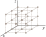
\includegraphics[scale=1]{figures/ch_18/fig_18_40.pdf}
            % \caption[]{}
			\caption[]{Formation of diffraction maxima from a three-dimensional structure. The coordinate axes $x$, $y$ and $z$ are positioned in the directions along which the properties of the structure display periodicity.}
			\label{fig:18_40}
		\end{center}
	\end{minipage}
\vspace{-0.4cm}
\end{figure}

Any two-dimensional periodic structures such as a system of small apertures or one of opaque tiny spheres produce a diffraction pattern similar to that shown in \fig{18_39}.

For diffraction maxima to appear, it is essential that the period of the structure $d$ be greater than $\lambda$.
Otherwise, conditions \eqref{eq:18_56} and \eqref{eq:18_57} can be satisfied only at values of $m_1$ and $m_2$ equal to zero (the magnitude of $\sin\varphi$ cannot exceed unity).

Diffraction is also observed in three-dimensional structures, \ie, spatial formations displaying periodicity along three directions not in one plane.
All crystalline bodies are such structures. Their period ($\sim\SI{e-10}{\metre}$), however, is too small for the observation of diffraction in visible light.
The condition $d\lambda$ is observed for crystals only for X-rays.
The diffraction of X-rays from crystals was first observed in 1913 in an experiment conducted by the German physicists Max von Laue (1879-1959), Walter Friedrich (1883-1968), and Paul Knipping (1883-1935).
(The idea belonged to von Laue, while the other two authors ran the experiment.).

Let us find the conditions for the formation of diffraction maxima from a three-dimensional structure.
We position the coordinate axes $x$, $y$, and $z$ in the directions along which the properties of the structure display periodicity (\fig{18_40}).
The structure can be represented as a collection of equally spaced parallel trains of structural elements arranged along one of the coordinate axes.
We shall consider the action of an individual linear train parallel, for instance, to the $x$-axis (\fig{18_41}).
Assume that a beam of parallel rays making the angle $\alpha_0$ with the $x$-axis falls on the train.
Every structural element is a source of secondary wavelets.
An incident wave arrives at adjacent sources with a phase difference of $\delta_0=2\pi \Delta_0/\lambda$, where $\Delta_0=d_1 \cos\alpha_0$ (here, $d_1$ is the period of the structure along the $x$-axis).
Apart from this, the additional path difference $\Delta=d_1\cos\alpha$ is produced between the secondary wavelets propagating in directions that make the angle $\alpha$ with the $x$-axis (all such directions lie along the generatrices of a cone whose axis is the $x$-axis).
The oscillations from different structural elements will be mutually amplified for the directions for which
\begin{equation}\label{eq:18_58}
	d_1 (\cos\alpha - \cos\alpha_0) = \pm m_1 \lambda \quad (m_1 = 0,1,2,\ldots).
\end{equation}

\begin{figure}[t]
	\begin{center}
		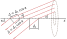
\includegraphics[scale=1.0]{figures/ch_18/fig_18_41.pdf}
		% \caption[]{}
        \caption[]{Scheme of a collection of equally spaced parallel trains of structural elements arranged along the $x$-axis.}
		\label{fig:18_41}
	\end{center}
	\vspace{-0.8cm}
\end{figure}

There is a separate cone of directions for each value of $m_1$, and along these directions we get maxima of the intensity from one individually taken train parallel to the $x$-axis.
The axis of this cone coincides with the $x$-axis.

The condition of the maximum for a train parallel to the $y$-axis has the form
\begin{equation}\label{eq:18_59}
	d_2 (\cos\beta - \cos\beta_0) = \pm m_2 \lambda \quad (m_2=0,1,2,\ldots),
\end{equation}

\noindent
where $d_2$ is the period of the structure in the direction of the $y$-axis, $\beta_0$ is the angle between the incident beam and the $y$-axis, and $\beta$ is the angle between the $y$-axis and the directions along which diffraction maxima are obtained.

A cone of directions whose axis coincides with the $y$-axis corresponds to each value of $m_2$.

In directions satisfying conditions \eqref{eq:18_58} and \eqref{eq:18_59} simultaneously, mutual amplification of the oscillations from sources in the same plane perpendicular to the $z$-axis occur (these sources form a two-dimensional structure).
The directions of the intensity maxima produced lie along the lines of intersection of the direction cones, of which one is determined by condition \eqref{eq:18_58}, and the second one by condition \eqref{eq:18_59}.

Finally, for the train parallel to the $z$-axis, the directions of the maxima are determined by the condition
\begin{equation}\label{eq:18_60}
	d_3 (\cos\gamma - \cos\gamma_0) = \pm m_3 \lambda \quad (m_3=0,1,2,\ldots),
\end{equation}

\noindent
where $d_3$ is the period of the structure in the direction of the $z$-axis, $\gamma_0$ is the angle between the incident beam and the $z$-axis, and $\gamma$ is the angle between the $z$-axis and the directions along which diffraction maxima are obtained.

As in the preceding cases, a cone of directions whose axis coincides with the $z$-axis corresponds to each value of $m_3$.

In the directions satisfying conditions \eqref{eq:18_58}, \eqref{eq:18_59}, and \eqref{eq:18_60} simultaneously, mutual amplification of the oscillations from all the elements forming the three-dimensional structure occurs.
As a result, diffraction maxima are produced by the three-dimensional structure.
The directions of these maxima are on the lines of intersection of three cones whose axes are parallel to the coordinate axes.

The conditions
\begin{align}
		d_1 (\cos\alpha - \cos\alpha_0) &= \pm m_1 \lambda, \nonumber\\
		d_2 (\cos\beta - \cos\beta_0) &= \pm m_2 \lambda, \quad (m_i=0,1,2,\ldots) \label{eq:18_61}\\
		d_3 (\cos\gamma - \cos\gamma_0) &= \pm m_3 \lambda, \nonumber
\end{align}

\noindent
which we have found are called \textbf{Laue's formulas}.
Three integral numbers $m_1$, $m_2$, and $m_3$ correspond to each direction ($\alpha$, $\beta$, $\gamma$) determined by these formulas.
The greatest value of the magnitude of the difference between cosines is two.
Hence, conditions \eqref{eq:18_61} can be obeyed with values of the numbers $m$ other than zero only provided that $\lambda$ does not exceed $2d$.

The angles $\alpha$, $\beta$ and $\gamma$ are not independent.
For example, when a Cartesian system of coordinates is used, they are related by the expression
\begin{equation}\label{eq:18_62}
	\cos^2\alpha + \cos^2\beta + \cos^2\gamma = 1.
\end{equation}

\noindent
Thus, when $\alpha_0$, $\beta_0$ and $\gamma_0$ are given, the angles $\alpha$, $\beta$ and $\gamma$ determining the directions of the maxima can be found by solving a system of four
equations.
If the number of equations exceeds the number of unknowns, a system of equations can be solved only when definite conditions are observed (only when these conditions are satisfied can the three cones intersect one another along a single line).

The system of \eqns{18_61}{18_62} can be solved only for certain quite definite wavelengths ($\lambda$ can be considered as a fourth unknown whose values obtained from the solution of the system of equations are exactly the wavelengths for which maxima are observed).
Generally speaking, only one maximum corresponds to each such value of $\lambda$.
Several symmetrically arranged maxima may be obtained, however.

If the wavelength is fixed (monochromatic radiation), the system of equations can be made simultaneous by varying the values of $\alpha_0$, $\beta_0$ and $\gamma_0$, \ie, by turning the three-dimensional structure relative
to the direction of the incident beam.

We have not treated the question of how rays travelling from different structural elements are made to converge to one point on a screen.
A lens does this for visible light.
A lens cannot be used for X-rays because the refractive index of these rays in all substances
is virtually equal to unity.
For this reason, the interference of the secondary wavelets is achieved by using very narrow beams of rays producing spots of a very small size on a screen (or a photographic plate) even without a lens.

The Russian scientist Yuri Vulf (1863-1925) and the British physicists William Henry Bragg (1862-1942) and his son William Lawrence Bragg (1890-1971) showed independently of each other that the diffraction pattern from a crystal lattice can be calculated in the following simple way. Let us draw parallel equispaced planes through the points of a crystal lattice (\fig{18_42}).
We shall call these planes atomic layers.
If the wave falling on the crystal is plane, the envelope of the secondary waves set up by the atoms in such a layer will also be a plane.
Thus, the summary action of the atoms in one layer can be represented in the form of a plane wave reflected from an atom-covered surface according to the usual law of reflection.

The plane secondary wavelets reflected from different atomic layers are coherent and will interfere with one another like the waves emitted in the given direction by different slits of a diffraction grating.
As in the case of a grating, the secondary wavelets will virtually destroy one another in all directions except those for which the path difference between adjacent wavelets is a multiple of $\lambda$.
Inspection of \fig{18_42} shows that the difference between the paths of two waves reflected from adjacent atomic layers is $2d\sin\theta$, where $d$ is the period of identity of the crystal in a direction at right angles to the layers being considered, and $\theta$ is the angle supplementing the angle of incidence and called the \textbf{glancing angle} of the incident rays.
Consequently, the directions in which diffraction maxima are obtained are determined by the condition
\begin{equation}\label{eq:18_63}
	2d \sin\theta = \pm m \lambda \quad (m=0,1,2,\ldots).
\end{equation}

\noindent
This expression is known as the \textbf{Bragg-Vulf} formula.

\begin{figure}[t]
	\begin{minipage}[t]{0.48\linewidth}
		\begin{center}
			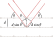
\includegraphics[scale=1]{figures/ch_18/fig_18_42.pdf}
			% \caption[]{}
            \caption[]{Reflection of a plane wave upon parallel equispaced planes through the points of a crystal lattice (atomic planes). $d$ is the period of identity of the crystal and $\theta$ is the angle supplementing the angle of incidence and called the glancing angle of the incident rays.}
			\label{fig:18_42}
		\end{center}
	\end{minipage}
	\hfill{ }%space{-0.05cm}
	\begin{minipage}[t]{0.48\linewidth}
		\begin{center}
			\includegraphics[scale=1]{figures/ch_18/fig_18_43.pdf}
            % \caption[]{}
			\caption[]{The difference between the paths of two waves reflected from adjacent atomic layers is $2d \sin\theta$. ($d$ and $theta$ are described in the caption of \fig{18_42}).}
			\label{fig:18_43}
		\end{center}
	\end{minipage}
\vspace{-0.4cm}
\end{figure}

The atomic layers in a crystal can be drawn in a multitude of ways (\fig{18_43}).
Each system of layers can produce a diffraction maximum if condition \eqref{eq:18_63} is observed for it.
Only those maxima have an appreciable intensity, however, that are obtained as a result of reflections from layers sufficiently densely populated by atoms (for instance, from layers I and II in \fig{18_43}).

We must note that calculations by the Bragg-Vulf formula and by Laue's formulas [see Eqs. \eqref{eq:18_61}] lead to coinciding results.

The diffraction of X-rays from crystals has two principal applications.
It is used to investigate the spectral composition of X-radiation (\textbf{X-ray spectroscopy}) and to study the structure of crystals (\textbf{X-ray structure analysis}).

By determining the directions of the maxima obtained in the diffraction of the X-radiation being studied from crystals with a known structure, we can calculate the wavelengths.
Originally, crystals of the cubic system were used to determine wavelengths, the spacing of the
planes being determined from the density and relative molecular mass of the crystal.

In the method of structural analysis proposed by von Laue, a beam of X-rays is directed onto
a stationary monocrystal.
The radiation contains a wavelength at which condition \eqref{eq:18_63} is satisfied for each system of layers sufficiently densely populated by atoms.
Consequently, we obtain a collection of black spots on a photographic plate placed behind the crystal (after development).
The mutual arrangement of the spots reflects the symmetry of the crystal.
The distances between the spots and their intensities allow us to find the arrangement of the atoms in a crystal and their spacing.
Figure \ref{fig:18_44} shows a Laue diffraction pattern of beryl (a mineral of the silicate group).

\begin{figure}[t]
	\begin{center}
		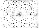
\includegraphics[scale=1.0]{figures/ch_18/fig_18_44.pdf}
		% \caption[]{}
        \caption[]{Laue diffraction pattern of beryl (a mineral of the silicate group).}
		\label{fig:18_44}
	\end{center}
	\vspace{-0.8cm}
\end{figure}

The method of structural analysis developed by the Dutch physicist Peter Debye and the Swiss physicist Paul Scherrer uses monochromatic X-radiation and polycrystalline specimens.
The substance being studied is ground into a powder, and the latter is pressed into a wire-shaped specimen.
The specimen is put along the axis of a cylindrical chamber on whose side surface a photographic film is placed (\fig{18_45}).
Among the enormous number of chaotically oriented minute crystals, there will always be a multitude of such ones for which condition \eqref{eq:18_63} will be observed, the diffracted ray being in the most diverse planes for different crystals.
As a result, for each system of atomic layers and each value of $m$, we get not one direction of a maximum, but a cone of directions whose axis
coincides with the direction of the incident beam (see \fig{18_45}).
The pattern obtained on the film (a Debye powder pattern) has the form shown in \fig{18_46}.
Each pair of symmetrically arranged lines corresponds to one of the diffraction maxima satisfying condition \eqref{eq:18_63} at a certain value of $m$.
The structure of the crystal can be determined by decoding the X-ray pattern.

\begin{figure}[t]
	\begin{center}
		\includegraphics[scale=1.0]{figures/ch_18/fig_18_45.pdf}
		% \caption[]{}
        \caption[]{Scheme of the instrument developed by Debye and Scherrer for structural analysis. It uses monochromatic X-radiation and polycrystalline specimens put along the axis of a cylindrical chamber on whose side surface a photographic film is placed.}
		\label{fig:18_45}
	\end{center}
	\vspace{-0.2cm}
\end{figure}


\begin{figure}[t]
	\begin{center}
		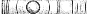
\includegraphics[scale=1.0]{figures/ch_18/fig_18_46.pdf}
		% \caption[]{}
        \caption[]{Pattern obtained on the film (a Debye powder pattern). Each pair of symmetrically arranged lines corresponds to one of the diffraction maxima satisfying condition \eqref{eq:18_63} at a certain value of $m$.}
		\label{fig:18_46}
	\end{center}
	\vspace{-0.8cm}
\end{figure}

\section{Resolving Power of an Objective}\label{sec:18_8}

Assume that a plane light wave falls on an opaque screen with a round aperture of radius $b$ cut out of it.
The number of Fresnel zones opened by the aperture for point P opposite the centre of the
aperture at the distance $l$ from it can be found by \eqn{18_13} assuming that $a=\infty$, $r_0=b$, and $b=l$.
The result is
\begin{equation}\label{eq:18_64}
	m = \frac{b^2}{l \lambda}
\end{equation}

\noindent
[compare with expression \eqref{eq:18_37}].

In the same way as for a slit, depending on the value of parameter \eqref{eq:18_64}, we have to do either with the approximation of geometrical optics, or Fresnel diffraction, or, finally, Fraunhofer diffraction [see expressions \eqref{eq:18_36}].

We can observe a Fraunhofer diffraction pattern from a round aperture on a screen in the focal plane of a lens placed behind the aperture by directing a plane light wave onto the aperture.
This pattern has the form of a central bright spot surrounded by alternating dark and bright rings (\fig{18_47}).
The corresponding calculations show that the first minimum is at the angular distance from the centre of the diffraction pattern of
\begin{equation}\label{eq:18_65}
	\ab{\varphi}{min} = \arcsin\parenthesis{1.22\frac{\lambda}{D}},
\end{equation}

\noindent
where $D$ is the diameter of the aperture [compare with \eqn{18_28}].
If $D\gg\lambda$, we may consider that
\begin{equation}\label{eq:18_66}
	\ab{\varphi}{min} = 1.22 \frac{\lambda}{D}.
\end{equation}

\begin{figure}[t]
	\begin{center}
		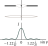
\includegraphics[scale=1.0]{figures/ch_18/fig_18_47.pdf}
		% \caption[]{}
        \caption[]{Fraunhofer diffraction pattern from a round aperture on a screen in the focal plane of a lens placed behind the aperture by directing a plane light wave onto the aperture. This pattern has the form of a central bright spot surrounded by alternating dark and bright rings.}
		\label{fig:18_47}
	\end{center}
	\vspace{-0.8cm}
\end{figure}

The major part (about $84\%$) of the light flux passing through the aperture gets into the region of the central bright spot.
The intensity of the first bright ring is only
$1.74\%$, and of the second, $0.41\%$ of the intensity of the central spot.
The intensity of the other bright rings is still
smaller.
For this reason, in a first approximation, we may consider that the diffraction pattern consists of only a single bright spot with an angular radius determined by \eqn{18_65}.
This spot is in essence the image of an infinitely remote point source of light (a plane light wave falls on the aperture).

The diffraction pattern does not depend on the distance between the aperture and the lens.
In particular, it will be the same when the edges of the aperture are made to coincide with the edges of the lens.
It thus follows that even a perfect lens cannot produce an ideal optical image.
Owing to the wave nature of light, the image of a point produced by the lens has the form of a spot that is the central maximum of a diffraction pattern.
The angular dimension of this spot diminishes with an increasing diameter of the lens mount $D$.

With a very small angular distance between two points, their images obtained with the aid of an optical instrument will be superposed and will produce a single luminous spot.
Hence, two very close points will not be perceived by the instrument separately or, as we say, will not be resolved by the instrument.
Consequently, no matter how great the image is in size, the corresponding details will not be seen on it.

Let $\delta\psi$ stand for the smallest angular distance between two points at which they can still be resolved by an optical instrument.
The reciprocal of $\delta\psi$ is called the \textbf{resolving power of the instrument}:
\begin{equation}\label{eq:18_67}
	R = \frac{1}{\delta\psi}.
\end{equation}

\begin{figure}[t]
	\begin{center}
		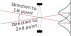
\includegraphics[scale=0.9]{figures/ch_18/fig_18_48.pdf}
		% \caption[]{}
        \caption[]{Rayleigh criterion: two close points will still be resolved if the middle of the central diffraction maximum for one of them coincides with the edge of the central maximum for the second one. This occurs if the angular distance between the points $\delta\psi$ equals the angular radius given by \eqn{18_65}.}
		\label{fig:18_48}
	\end{center}
	\vspace{-0.8cm}
\end{figure}

Let us find the resolving power of the objective of a telescope or camera when very remote objects are being looked at or photographed.
In this condition, the rays travelling into the objective from each point of the object may be considered parallel, and we can use formula \eqref{eq:18_65}.
According to the Rayleigh criterion, two close points will still be resolved if the middle of the central diffraction maximum for one of them coincides with the edge of the central maximum (\ie, with the first minimum) for the second one.
A glance at \fig{18_48} shows that this will occur if the angular distance between the points $\delta\psi$ will equal the angular radius given by \eqn{18_65}.
The diameter of the objective mount $D$ is much greater than the wavelength $\lambda$.
We may therefore consider that
\begin{equation*}
	\delta\psi = 1.22 \frac{\lambda}{D}.
\end{equation*}

\noindent
Hence,
\begin{equation}\label{eq:18_68}
	R = \frac{D}{1.22 \lambda}.
\end{equation}

\noindent
It can be seen from this formula that the resolving power of an objective grows with its diameter.

The diameter of the pupil of an eye at normal illumination is about \SI{2}{\milli\metre}.
Using this value in \eqn{18_68} and taking $\lambda = \SI{0.5e-3}{\milli\metre}$, we get
\begin{equation*}
	\delta\psi = 1.22 \times \frac{\num{0.5e-3}}{2} = \SI{0.305e-3}{\radian} \approx \ang{;1;}.
\end{equation*}

\noindent
Thus, the minimum angular distance between points at which the human eye still perceives them separately, equals one angular minute.
It is interesting to note that the distance between adjacent light sensitive elements of the retina corresponds to this angular distance.

\section{Holography}\label{sec:18_9}

Holography (\ie, ``complete recording'', from the Greek ``bolos'' meaning ``the whole'' and ``grapho''-``write'') is a special way of recording the structure of the light wave reflected by an object on a photographic plate.
When this plate (a hologram) is illuminated with a beam of light, the wave recorded on it is reconstructed in practically its original form, so that when the eye perceives the reconstructed wave, the visual sensation is virtually the same as it would be if the object itself were observed.

Holography was invented in 1947 by the British physicist Dennis Gabor.
The complete embodiment of Gabor's idea became possible, however, only after the appearance
in 1960 of light sources having a high degree of coherence---lasers.
Gabor's initial arrangement was improved by
the American physicists Emmet Leith and Juris Upatnieks, who obtained the first laser holograms in 1963.
The Soviet scientist Yuri Denisyuk in 1962 proposed an original method of recording holograms on a thick-layer emulsion.
This method, unlike holograms on a thin-layer emulsion, produces a coloured image of the object.

We shall limit ourselves to an elementary consideration of the method of recording holograms on a thin-layer emulsion.
Figure \ref{fig:18_49}a contains a schematic view of an arrangement for recording holograms,
and \fig{18_49}b a schematic view of reconstruction of the image.
The light beam emitted by the laser, expanded by a system of lenses, is split into two parts.
One part is reflected by the mirror to the photographic plate forming the so-called reference wave $1$.
The second part reaches the plate after being reflected from the object; it forms object beam $2$.
Both beams must be coherent.
This requirement is satisfied because laser radiation has a high degree of spatial coherence (the light oscillations are coherent over the entire cross section of a laser beam).
The reference and object beams superpose and form an interference pattern that is recorded by the photographic plate.
A plate exposed in this way and developed is a \textbf{hologram}.
Two beams of light participate in forming the hologram.
In this connection, the arrangement described above is called two-beam or split-beam holography.

\begin{figure}[t]
	\begin{center}
		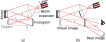
\includegraphics[scale=1]{figures/ch_18/fig_18_49.pdf}
		% \caption[]{}
        \caption[]{Holograms on a thin-layer emulsion. (a) Schematic view of an arrangement for recording holograms. (b) Schematic view of reconstruction of the image.}
		\label{fig:18_49}
	\end{center}
	\vspace{-0.8cm}
\end{figure}

To reconstruct the image, the developed photographic plate is put in the same place where it was in recording the hologram, and is illuminated with the reference beam of light (the part of the laser beam that illuminated the object in recording the hologram is now stopped).
The reference beam diffracts on the hologram, and as a result a wave is produced having exactly the same structure as the one reflected by the object.
This wave produces a virtual image of the object that is seen by the observer.
In addition to the wave forming the virtual image, another wave is produced that gives a real
image of the object.
This image is pseudoscopic; this means that it has a relief which is the opposite of the relief of the $2$ object---the convex spots are replaced by concave ones, and vice versa.

Let us consider the nature of a hologram and the process of image reconstruction.
Assume that two coherent parallel beams of light rays fall on the photographic plate, with the angle $\psi$ between the beams (\fig{18_50}).
Beam $1$ is the reference one, and beam $2$, the object one (the object in the given case is an infinitely remote point).
We shall assume for simplicity that beam $1$ is normal to the plate.
All the results obtained below also hold when the reference beam falls at an angle, but the formulas will be more cumbersome.

% \begin{figure}[t]
% 	\begin{center}
% 		\includegraphics[scale=1]{figures/ch_18/fig_18_50.pdf}
% 		% \caption[]{}
%         \caption[]{Two coherent parallel beams of light rays fall on the photographic plate, with the angle $\psi$ between the beams. Beam $1$ is the reference one, and beam $2$, the object one (the object is considered an infinitely remote point).}
% 		\label{fig:18_50}
% 	\end{center}
% 	\vspace{-0.8cm}
% \end{figure}

\begin{figure}[t]
	\begin{minipage}[t]{0.48\linewidth}
		\begin{center}
			\includegraphics[scale=1]{figures/ch_18/fig_18_50.pdf}
			% \caption[]{}
	        \caption[]{Two coherent parallel beams of light rays fall on the photographic plate, with the angle $\psi$ between the beams. Beam $1$ is the reference one, and beam $2$, the object one (the object is considered an infinitely remote point). We shall assume for simplicity that beam $1$ is normal to the plate.}
			\label{fig:18_50}
		\end{center}
	\end{minipage}
	\hfill{ }%space{-0.05cm}
	\begin{minipage}[t]{0.48\linewidth}
		\begin{center}
			\includegraphics[scale=1]{figures/ch_18/fig_18_51.pdf}
			% \caption[]{}
	        \caption[]{Plate illuminated with a reference beam, produces a diffraction pattern whose maxima form the angles $\varphi$ with a normal to the plate. The maximum corresponding to $m=0$ is on the continuation of the reference beam. The maximum corresponding to $m=+1$ has the same direction as object beam $2$ did during the exposure. In addition, a maximum corresponding to $m=-1$ appears.}
			\label{fig:18_51}
		\end{center}
	\end{minipage}
\vspace{-0.4cm}
\end{figure}

Owing to the interference of the reference and object beams, a system of alternating straight maxima and minima of the intensity is formed on the plate.
Let points A and B correspond to the middles of adjacent interference maxima.
Hence, the path difference $\Delta'$ equals $\lambda$.
Examination of \fig{18_50} shows that $\Delta'= d\sin\psi$; hence,
\begin{equation}\label{eq:18_69}
	d \sin\psi = \lambda.
\end{equation}

Having recorded the interference pattern on the plate (by exposure and developing), we direct reference beam $1$ at it.
For this beam, the plate plays the part of a diffraction grating whose period $d$ is determined by \eqn{18_69}.
A feature of this grating is the circumstance that its transmittance changes in a direction perpendicular to the ``lines'' according to a cosine law (in the gratings treated in \sect{18_6} it changed in a jump: gap-dark-gap-dark, etc.).
The result of this feature is that the intensity of all the diffraction maxima of orders higher than the first one virtually equals zero.

When the plate is illuminated with the reference beam (\fig{18_51}), a diffraction pattern appears whose maxima form the angles $\varphi$ with a normal to the plate.
These angles are determined by the condition
\begin{equation}\label{eq:18_70}
	d \sin\varphi = m \lambda \quad (m=0, \pm 1)
\end{equation}

\noindent
[compare with formula \eqref{eq:18_41}].
The maximum corresponding to $m=0$ is on the continuation of the reference beam.
The maximum corresponding to $m=\pm 1$ has the same direction as object beam $2$ did during the exposure [compare \eqns{18_69}{18_70}].
In addition, a maximum corresponding to $m=-1$ appears.

% \begin{figure}[t]
% 	\begin{center}
% 		\includegraphics[scale=1]{figures/ch_18/fig_18_51.pdf}
% 		% \caption[]{}
%         \caption[]{Plate illuminated with a reference beam, produces a diffraction pattern whose maxima form the angles $\varphi$ with a normal to the plate. The maximum corresponding to $m=0$ is on the continuation of the reference beam. The maximum corresponding to $m=+1$ has the same direction as object beam $2$ did during the exposure. In addition, a maximum corresponding to $m=-1$ appears.}
% 		\label{fig:18_51}
% 	\end{center}
% 	\vspace{-0.8cm}
% \end{figure}

It can be shown that the result we have obtained also holds when object beam $2$ consists of diverging rays instead of parallel ones.
The maximum corresponding to $m = +1$ has the nature of diverging beam of rays $2'$ (it produces a virtual image of the point from which
rays $2$ emerged during the exposure); the maximum corresponding to $m = -1$, on the other hand, has the nature of a converging beam of rays $2''$ (it forms a real image of the point which rays $2$ emerged from during the exposure).

In recording the hologram, the plate is illuminated by reference beam $1$ and numerous diverging beams $2$ reflected by different points of the object.
An intricate interference pattern is formed on the plate as a result of superposition of the patterns produced by each of the beams $2$ separately.
When the hologram is illuminated with reference beam $1$, all beams $2$ are reconstructed, \ie, the complete light wave reflected by the object ($m = +1$ corresponds to it).
Two other waves appear in addition to it (corresponding to $m = 0$ and $m = -1$).
But these waves propagate in other directions and do not hinder the perception of the wave producing a virtual image of the object (see \fig{18_49}).

The image of an object produced by a hologram is three-dimensional.
It can be viewed from different positions.
If in recording a hologram close objects concealed more remote ones, then by moving to a side we can look behind the closer object (more exactly, behind its image) and see the objects that had been concealed previously.
The explanation is that when moving to a side we see the image reconstructed from the peripheral part of the hologram onto which the rays reflected from the concealed objects also fell during the exposure.
When looking at the images of close and far objects, we have to accommodate our eyes as when looking at the objects themselves.

If a hologram is broken into several pieces, then each of them when illuminated will produce the same picture as the original hologram.
But the smaller the part of the hologram used to reconstruct the image, the lower is its sharpness.
This is easy to understand by taking into account that when the number of lines of a diffraction grating is reduced, its resolving power diminishes [see \eqn{18_55}].

The possible applications of holography are very diverse.
A far from complete list of them includes holographic motion pictures and television, holographic microscopes, and control of the quality of processing articles.
The statement can be encountered in publications on the subject that holography can be compared as regards its consequences with the setting up of radio communication.
